% !TeX program = xelatex
% 在本目录使用 XeLaTeX 编译两次。
\documentclass[UTF8,11pt,a4paper,oneside,openany,fontset=fandol]{ctexbook}
\usepackage[left=24mm,right=24mm,top=23mm,bottom=24mm,headheight=16pt]{geometry}
\usepackage{amsmath,amssymb,mathtools,bm,graphicx,booktabs,longtable,array,tabularx}
\usepackage{xcolor,enumitem,fancyhdr,listings,tikz}
\usetikzlibrary{arrows.meta,positioning,calc,fit}
\usepackage[unicode,colorlinks=true,linkcolor=black,citecolor=black,urlcolor=blue!40!black]{hyperref}
\definecolor{ink}{HTML}{253346}
\definecolor{accent}{HTML}{345B74}
\definecolor{papergray}{HTML}{F3F4F5}
\hypersetup{pdftitle={Ariadne 与 Ariadne-Xtal：从原始衍射像素到结构推断的数学与算法},pdfauthor={Ariadne 技术文档},pdfsubject={数学推导、实现边界与已有验证证据}}
\ctexset{chapter={format=\huge\bfseries\color{ink},beforeskip=0pt,afterskip=20pt},section={format=\Large\bfseries\color{ink}}}
\setlength{\parindent}{2em}\setlength{\parskip}{3pt}
\setlength{\emergencystretch}{3em}\renewcommand{\arraystretch}{1.18}
\linespread{1.10}\allowdisplaybreaks
\setcounter{tocdepth}{1}\setcounter{secnumdepth}{2}
\setlist{itemsep=3pt,topsep=5pt,leftmargin=2em}
\pagestyle{fancy}\fancyhf{}
\fancyhead[L]{\small Ariadne / Ariadne-Xtal}
\fancyhead[R]{\small 数学、算法与证据}
\fancyfoot[C]{\thepage}\renewcommand{\headrulewidth}{0.3pt}
\newcommand{\vct}[1]{\bm{#1}}\newcommand{\mat}[1]{\mathbf{#1}}
\newcommand{\iu}{\mathrm{i}}\newcommand{\dif}{\mathrm{d}}\newcommand{\E}{\mathbb E}
\newcommand{\Var}{\operatorname{Var}}\newcommand{\Cov}{\operatorname{Cov}}
\newcommand{\tr}{\operatorname{tr}}\newcommand{\rank}{\operatorname{rank}}
\newcommand{\diag}{\operatorname{diag}}\newcommand{\Real}{\operatorname{Re}}
\newcommand{\Imag}{\operatorname{Im}}\newcommand{\argmin}{\operatorname*{arg\,min}}
\newcommand{\angstrom}{\text{\AA}}\newcommand{\code}[1]{{\small\nolinkurl{#1}}}
\newcommand{\latinfont}{\rmfamily}
\newenvironment{principle}{\begin{quote}\small\color{ink}}{\end{quote}}
\lstset{basicstyle=\footnotesize\ttfamily,breaklines=true,columns=fullflexible,keepspaces=true,showstringspaces=false,frame=single,rulecolor=\color{black!15},backgroundcolor=\color{papergray}}
\renewcommand{\topfraction}{0.88}\renewcommand{\bottomfraction}{0.8}
\renewcommand{\textfraction}{0.1}\renewcommand{\floatpagefraction}{0.8}
\begin{document}
\frontmatter
\begin{titlepage}
\vspace*{15mm}
{\large\color{accent} 数学与算法技术报告\par}
\vspace{15mm}
{\Huge\bfseries Ariadne 与 Ariadne-Xtal\par}
\vspace{8mm}
{\LARGE\bfseries 从原始衍射像素到结构推断\par}
\vspace{10mm}
{\large 探测器还原、自校准检测、重叠积分、相位恢复与约束精修\par}
\vspace{12mm}\noindent\rule{\textwidth}{0.6pt}
\vspace{5mm}
本报告以用户提供的\textit{单晶结构求解与精修的数学基础}为参考，保留散射物理与结构推断主线，补充 Ariadne 数据还原算法、精确加速及现有实测证据。
\vfill
\noindent\begin{tabularx}{\textwidth}{@{}lX@{}}
报告日期 & 2026 年 11 月 01 日\\
源码基线 & Ariadne 0.7.0；提交 \code{cec63ba186a1843389b1ae161944388304ff1cdd}\\
还原接口 & DIALS 3.30.1 源码扩展及进程内 Bruker100 适配\\
结构模块 & 独立 Ariadne-Xtal 原生算法与显式 SHELXT/SHELXL 后端\\
证据口径 & 已保存的数值记录与源码核对；本次未重跑科学基准\\
\end{tabularx}
\end{titlepage}
\chapter*{内容提要}\addcontentsline{toc}{chapter}{内容提要}
单晶衍射分析的核心是从有限、带噪声的强度观测推断周期结构。原始像素的单位、背景与相关噪声决定弱信号是否可见；晶格几何和轮廓决定重叠反射能否区分；相位缺失、对称性和参数相关性决定原子模型是否可辨识。Ariadne 与 Ariadne-Xtal 分别实现这些问题中的数据还原与结构计算部件，并通过有类型的产物与来源记录衔接。

本报告先由电子散射、晶胞度量和概率模型建立统一正向关系，再推导原始 ADU 还原、自校准 matched-filter、周期晶格密度评分、共享像素积分、Gaussian 增广 QR 压缩及条件剖面区间。随后讨论相位恢复、非线性精修、严格约束、化学限制、无序、孪晶与不确定度，并给出结构反馈的信息上限、低秩条件化及防止数据重复使用的分组规则。

现有记录表明，自校准检测在指定合成留出场景中提高召回率与 F1，精确率略低于获得真实噪声方差图的 DIALS 强基线；四工作单元检测仍比 DIALS C++ 内核慢约 3.12 倍。固定方差 Gaussian 约束积分在 12,000 与 60,000 行合成像素组中分别加速约 3.62 与 11.41 倍。32 帧真实数据已完成 import 至 integrate 的软件衔接，但完整多扫描、多域结构解析尚未建立科学验收。结构模块与真实 SHELXL 的有限受控比较给出接近的精修指标，其范围不覆盖全部 SHELX 指令。

报告将数学恒等式、近似模型、源码行为和既有验证分开叙述。这里给出的精度和时间均对应明确案例；公式成立的前提与计算成功的含义同时给出，以便读者判断哪些量来自测量，哪些量依赖模型。
\chapter*{阅读约定}\addcontentsline{toc}{chapter}{阅读约定}
倒易基矢不含 $2\pi$；长度为 $\angstrom$，笛卡尔位移张量为 $\angstrom^2$。结构因子使用正指数，电子密度反变换使用负指数。原始 ADU、DIALS corrected 像素、光子等效值和校正后的积分强度分别定义，不能仅凭数值相近互换。

参考 PDF 的理论章节在本报告中整理、复用，并据当前实现补注。已有图版沿用原报告明确标注的合成示例；本次没有生成新的科学实验结果。证据文件是本地保存的历史记录，报告制作只执行文档编译和排版检查。

源码中 $A$ 的历史命名有时指晶胞、有时指取向后的倒易基。为避免歧义，本报告新写的数据还原章节以 $C$ 表示直接晶胞矩阵，以 $A_q=UC^{-\mathsf T}$ 表示取向后的倒易基；沿用的结构章节仍用 $\mat A$ 表示直接晶胞，其局部定义优先。
\tableofcontents
\chapter*{主要符号}\addcontentsline{toc}{chapter}{主要符号}
\begin{longtable}{p{32mm}p{106mm}}
\toprule 符号 & 定义与单位\\\midrule\endfirsthead
\toprule 符号 & 定义与单位\\\midrule\endhead
$C,\mat A$ & 直接晶胞矩阵，列为基矢，$\angstrom$\\
$B=C^{-\mathsf T},A_q=UB$ & 倒易基及取向后的倒易基，$\angstrom^{-1}$\\
$\vct h,\vct x,\vct r$ & Miller 指数、分数坐标与笛卡尔坐标\\
$Y,g,o,v_r$ & 原始 ADU、ADU/count 增益、ADU 偏置、ADU$^2$ 读出方差\\
$x,b,r$ & 光子等效像素、背景、该单位下的读出方差\\
$h,H$ & 一维检测核与二维可分离检测核；$H$ 在反馈章节也表示观测设计矩阵\\
$\rho_d,\kappa_H,\phi$ & 残差相关、核方差修正与局部超额方差因子\\
$P,I,B_0\beta$ & 轮廓设计、完整轮廓强度与像素背景\\
$F_h,\mu_h,y_h$ & 复结构因子、预测强度与有符号观测强度\\
$o_j,U_j,\alpha_d$ & 物理占有率、位移协方差与孪晶畴分数\\
$J,C_p$ & 残差 Jacobian 与条件参数协方差\\
$m,C_m,D+UU^{\mathsf T}$ & 结构强度预测、其协方差及低秩表示\\
\bottomrule
\end{longtable}
\mainmatter
\chapter{统一问题与算法交付范围}
\section{从观测到结构的正向关系}
设几何参数为 $\eta$，原子模型为 $p$，第 $a$ 个反射的完整强度为 $I_a$。一个像素的物理模型可写为
\begin{align}
N_j&\sim\mathrm{Poisson}\left(b_j+\sum_a P_{ja}(\eta)I_a\right),\\
Y_j&=o_j+g_jN_j+\epsilon_j,\qquad \epsilon_j\sim N(0,v_{r,j}),\\
I_h^{\rm ideal}&=k\sum_d\alpha_d\left|F_{T_dh}(p)\right|^2.
\end{align}
这里的 $P_{ja}$ 包含探测器像素与扫描角度内的轮廓质量，$T_d$ 描述相应畴的反射映射。几何、噪声、强度与原子参数处于不同层次：检测返回候选像素，积分返回幅度及相关误差，结构计算解释校正后的强度。测量模型中的 $I_a$ 与结构模型中的 $I_h^{\rm ideal}$ 之间还需要明确尺度、吸收、Lorentz、偏振和观测组合关系。

完整联合推断可以写为 $-\log p(Y\mid I,\eta)-\log p(I\mid p)-\log p(p,\eta)$。当前代码以模块化条件求解实现其中若干部件；没有把这一形式整体求到全局最优，也没有同时传播所有仪器、背景、轮廓和结构不确定度。
\section{系统分工与完成标准}
\begin{table}[htbp]\centering\small
\begin{tabularx}{\textwidth}{p{25mm}XX}
\toprule 层次 & 输出与职责 & 当前实现范围\\\midrule
Ariadne 还原 & 候选像素、晶格、轮廓、积分与导出 & DIALS 源码扩展、原始读取适配和独立科学脚本\\
Ariadne-Xtal & 散射、相位候选、约束精修、地图 & 已知组成的原生 $P1$ 求相位及明确支持的结构模型\\
官方结构后端 & SHELXT/SHELXL 原始指令行为 & 显式调用独立安装程序，不计为原生重实现\\
执行与证据 & 任务依赖、运行目录、产物来源与判断 & 执行成功、数值收敛、可辨识与科学接受分别记录\\
\bottomrule
\end{tabularx}
\caption{相互衔接而具有独立模型边界的计算层。}
\end{table}
一个完整技术结论需要同时说明输入、模型、数值结果与评价口径。例如，“检测 F1 提高”需要已知真值和一致组件提取；“积分分量可测”需要轮廓设计矩阵支持该对比；“结构已接受”需要化学、对称性、残余密度和独立证据。进程退出码不能替代这些判断。
\section{理论、实现与验证的对应}
理论部分说明一般关系，随后注明其在源码中的具体形式。相位章节的 Sayre 关系用于解释直接法原理，原生代码并未实现完整关系网络；精修章节的解析导数用于解释灵敏度，当前通用优化器仍以三点差分构造 Jacobian；反馈章节的交叉拟合规则是避免重复用数的必要设计，其低层来源字符串本身不能证明上游已执行排除。

本报告不修改原始帧、实测反射表或既有结构结果，也不包含实测反射表的发布包。性能与验证章节读取的是已经保存的结果，数学推导和文档排版不产生新的实验验收。

\chapter{从电子散射到晶胞结构因子}
\label{ch:scattering}
\section{单电子的弹性散射}
设入射 X 射线为频率 $\omega$、偏振矢量 $\vct e$ 的平面波。在远离吸收边、忽略电子束缚对弹性散射的主要修正时，电子受电场作用作受迫振动。非相对论运动方程为
\begin{equation}
m_e\ddot{\vct r}=-e\vct E_0 e^{-\iu\omega t},\qquad
\ddot{\vct r}=-\frac{e}{m_e}\vct E_0 e^{-\iu\omega t}.
\end{equation}
加速电荷产生辐射。远场振幅与入射场振幅之比包含经典电子半径
\begin{equation}
r_e=\frac{e^2}{4\pi\varepsilon_0m_ec^2}.
\end{equation}
对入射与散射偏振方向取投影后，单电子的微分散射截面为
\begin{equation}
\frac{\dif\sigma}{\dif\Omega}=r_e^2
\left|\vct e_{\mathrm{out}}^{*}\cdot\vct e_{\mathrm{in}}\right|^2.
\end{equation}
对两个相互垂直的入射偏振等权平均，并对未分析的两种出射偏振求和，即得到通常的非偏振因子 $(1+\cos^22\theta)/2$。该因子描述探测方向的几何响应，不属于晶体内部的电子密度。

令入射和出射波矢分别为 $\vct k_{\mathrm{in}}$、$\vct k_{\mathrm{out}}$，其长度均为 $2\pi/\lambda$。取散射矢量
\begin{equation}
\vct q=\vct k_{\mathrm{in}}-\vct k_{\mathrm{out}},\qquad
\lVert\vct q\rVert=\frac{4\pi\sin\theta}{\lambda}.
\end{equation}
位置 $\vct r$ 上的电子相对于原点多出相位 $\vct q\cdot\vct r$。在运动学近似下，各电子的散射振幅线性相加。

\section{电子密度的傅里叶表示}
若连续电子数密度为 $\rho(\vct r)$，以单电子振幅为单位的散射振幅为
\begin{equation}
F(\vct q)=\int\rho(\vct r)e^{\iu\vct q\cdot\vct r}\dif^3\vct r.
\label{eq:continuousF}
\end{equation}
这一关系来自相位叠加，不需要预先假定原子位置。原子模型只是对密度的一种参数化：
\begin{equation}
\rho(\vct r)=\sum_j o_j\rho_j(\vct r-\vct r_j).
\end{equation}
把该式代入式~\eqref{eq:continuousF}，并令 $\vct u=\vct r-\vct r_j$，得到
\begin{equation}
F(\vct q)=\sum_j o_j f_j(\vct q)e^{\iu\vct q\cdot\vct r_j},\qquad
f_j(\vct q)=\int\rho_j(\vct u)e^{\iu\vct q\cdot\vct u}\dif^3\vct u.
\end{equation}
当电子云近似球对称时，$f_j$ 只依赖 $s=\sin\theta/\lambda$。程序采用公开的 IT92 参数，由 Gemmi 提供系数~\cite{gemmi_scattering}：
\begin{equation}
f_j^0(s)=\sum_{m=1}^{4}a_{jm}e^{-b_{jm}s^2}+c_j.
\label{eq:it92}
\end{equation}
这些系数是散射曲线的数值近似，$\sum_ma_{jm}+c_j$ 可以略偏离原子序数。实现保持表值，不把这种偏差隐藏在额外的归一化中。

靠近吸收边时，散射包含色散修正：
\begin{equation}
f_j(s,\lambda)=f_j^0(s)+f'_j(\lambda)+\iu f''_j(\lambda).
\label{eq:anomalous}
\end{equation}
其中 $f'$ 改变与入射波同相的部分，$f''$ 描述相位相差 $\pi/2$ 的部分。在不同元素组成的非中心对称结构中，它们可使 $|F_{\vct h}|\ne|F_{-\vct h}|$。因此，保留 Friedel 对的独立观测是绝对结构分析的前提之一。

\section{晶格求和与衍射条件}
设直接晶格为 $\vct R_{\vct n}=\mat A\vct n$，$\vct n\in\mathbb Z^3$。有限晶体的振幅可分解为
\begin{equation}
F_{\mathrm{crystal}}(\vct q)
=F_{\mathrm{cell}}(\vct q)\sum_{\vct n}e^{\iu\vct q\cdot\mat A\vct n}.
\end{equation}
对由 $N_a,N_b,N_c$ 个晶胞组成的长方体，晶格和在每一方向上都是有限几何级数，例如
\begin{equation}
\sum_{n=0}^{N_a-1}e^{\iu n\varphi_a}
=e^{\iu(N_a-1)\varphi_a/2}
\frac{\sin(N_a\varphi_a/2)}{\sin(\varphi_a/2)}.
\end{equation}
当 $\varphi_a,\varphi_b,\varphi_c$ 分别接近 $2\pi$ 的整数倍时，强度集中成窄峰。理想无限晶格的条件为
\begin{equation}
\mat A^{\mathsf T}\vct q=2\pi\vct h,
\qquad \vct q=2\pi\mat A^{-\mathsf T}\vct h.
\end{equation}
定义 $\mat B=\mat A^{-\mathsf T}$ 和 $\vct g_{\vct h}=\mat B\vct h$，可得
\begin{equation}
d_{\vct h}^{-1}=\lVert\vct g_{\vct h}\rVert,
\qquad 2d_{\vct h}\sin\theta=\lambda.
\end{equation}
原子位置写作 $\vct r_j=\mat A\vct x_j$ 后，结构因子的相位简化为
\begin{equation}
\vct q\cdot\vct r_j=2\pi\vct h^{\mathsf T}\vct x_j.
\end{equation}
这说明散射振幅中的原子位置相位用分数坐标计算，而热运动与距离可以用笛卡尔坐标计算；二者通过晶胞矩阵连接。

\section{热运动的特征函数}
令原子的瞬时位置为 $\vct r_j+\vct u_j$，其中 $\E[\vct u_j]=0$。时间平均的原子振幅包含
\begin{equation}
\E\left[e^{\iu\vct q\cdot\vct u_j}\right].
\end{equation}
若位移服从三维正态分布，协方差为 $\mat U_j=\E[\vct u_j\vct u_j^{\mathsf T}]$，完成平方后得到高斯分布的特征函数
\begin{equation}
\E\left[e^{\iu\vct q\cdot\vct u_j}\right]
=\exp\left(-\frac12\vct q^{\mathsf T}\mat U_j\vct q\right)
=\exp\left(-2\pi^2\vct g^{\mathsf T}\mat U_j\vct g\right).
\label{eq:dw}
\end{equation}
各向同性情况下 $\mat U_j=U_{\mathrm{iso},j}\mat I$，因而
\begin{equation}
T_j(s)=e^{-8\pi^2U_{\mathrm{iso},j}s^2},\qquad
B_j=8\pi^2U_{\mathrm{iso},j}.
\end{equation}
热运动降低高角散射振幅，且不同方向衰减不同。若数据只有很窄的分辨率范围，位移参数、占有率和尺度就容易相关，因为它们均能改变幅度。

\section{正向模型的最终形式}
把占有率、散射因子、热运动和对称位置合并，得到原生内核使用的振幅
\begin{equation}
F_{\vct h}=\sum_{j\in\mathrm{ASU}}o_j f_j(s)
\sum_{m\in\mathcal O_j}
\exp\left[-2\pi^2\vct g^{\mathsf T}\mat U_{jm}\vct g
+2\pi\iu\vct h^{\mathsf T}\vct x_{jm}\right].
\label{eq:fullF}
\end{equation}
$\mathcal O_j$ 是原子 $j$ 的不同对称位置集合，重复位置只计一次。运动学强度模型为 $\mu_{\vct h}=k|F_{\vct h}|^2$，其中 $k$ 吸收了实验尺度及已经约定的强度归一化。

吸收、消光、多重散射、探测器响应和积分轮廓不是同一类效应。它们在原始观测到 $y_{\vct h}$ 的链条中有各自的位置。只有数据预处理与精修模型的定义一致，$k|F|^2$ 才能与输入强度直接比较。

\chapter{晶胞度量与空间群}
\section{任意晶胞的坐标变换}
取 $\vct a$ 沿笛卡尔 $x$ 轴，$\vct b$ 位于 $xy$ 平面。晶胞矩阵可写为
\begin{equation}
\mat A=\begin{pmatrix}
a&b\cos\gamma&c\cos\beta\\
0&b\sin\gamma&c\dfrac{\cos\alpha-\cos\beta\cos\gamma}{\sin\gamma}\\
0&0&\dfrac{V}{ab\sin\gamma}
\end{pmatrix},
\end{equation}
其中
\begin{equation}
V=abc\sqrt{1+2\cos\alpha\cos\beta\cos\gamma
-\cos^2\alpha-\cos^2\beta-\cos^2\gamma}.
\end{equation}
根号中的量必须为正。若该量过小，坐标变换将病态；软件在建立晶胞对象时即检验这一条件。

直接度量和倒易度量分别为
\begin{equation}
\mat G=\mat A^{\mathsf T}\mat A,\qquad
\mat G^*=\mat G^{-1}=\mat B^{\mathsf T}\mat B.
\end{equation}
于是分数位移 $\Delta\vct x$ 的平方距离，以及晶面间距，满足
\begin{equation}
d^2=\Delta\vct x^{\mathsf T}\mat G\Delta\vct x,\qquad
d_{\vct h}^{-2}=\vct h^{\mathsf T}\mat G^*\vct h.
\end{equation}
逐坐标将分数位移折入 $[-1/2,1/2]$，对一般斜晶胞不保证得到最近镜像。正确问题是整数最优化
\begin{equation}
\vct n_* =\argmin_{\vct n\in\mathbb Z^3}
\lVert\mat A(\Delta\vct x-\vct n)\rVert^2.
\label{eq:cvp}
\end{equation}
利用上三角矩阵 $\mat A$，可自第三坐标向第一坐标作球形分支定界。先取一个可行整数向量得到当前最小半径，每一层只枚举使剩余平方距离不超过该半径的整数区间。该过程具有明确的界，而不依赖任意设定的相邻 27 个晶胞。

\section{空间群操作与倒易空间关系}
空间群操作写成 Seitz 形式 $g=(\mat R,\vct t)$：
\begin{equation}
\vct x'=\mat R\vct x+\vct t\pmod{\mathbb Z^3}.
\end{equation}
对有效晶体操作，$\mat R$ 必须保持晶胞度量，
\begin{equation}
\mat R^{\mathsf T}\mat G\mat R=\mat G.
\end{equation}
在笛卡尔坐标中，相应的正交矩阵为 $\mat Q=\mat A\mat R\mat A^{-1}$。对称等价位置的位移张量随位置共同旋转：
\begin{equation}
\mat U'=\mat Q\mat U\mat Q^{\mathsf T}.
\end{equation}

由密度不变性 $\rho(\mat R\vct x+\vct t)=\rho(\vct x)$，在结构因子积分中换元可得
\begin{align}
F_{\vct h}
&=e^{2\pi\iu\vct h^{\mathsf T}\vct t}F_{\mat R^{\mathsf T}\vct h},\\
F_{\mat R^{\mathsf T}\vct h}
&=e^{-2\pi\iu\vct h^{\mathsf T}\vct t}F_{\vct h}.
\label{eq:symF}
\end{align}
振幅和强度的变换规律并不相同。强度满足 $I_{\mat R^{\mathsf T}\vct h}=I_{\vct h}$，没有平移相位因子。因此，电子密度图与 Patterson 图必须采用不同的对称展开规则。

\section{系统消光的推导}
若某操作满足 $\mat R^{\mathsf T}\vct h=\vct h$，式~\eqref{eq:symF} 给出
\begin{equation}
\left[1-e^{-2\pi\iu\vct h^{\mathsf T}\vct t}\right]F_{\vct h}=0.
\end{equation}
当括号不为零时，反射必须消失。例如，沿 $b$ 轴的 $2_1$ 螺旋操作 $(-x,y+1/2,-z)$ 对 $0k0$ 的作用为
\begin{equation}
F_{0k0}=e^{-\pi\iu k}F_{0k0},
\end{equation}
故 $k$ 为奇数时 $F_{0k0}=0$。对于体心平移 $(1/2,1/2,1/2)$，同样得到 $h+k+l=2n$。

消光条件是对空间群的必要约束，通常不是充分约束。不同空间群可以有相同的消光，弱反射、伪对称和重原子主导也可影响基于强度的判断。SHELXT 将相位求解与空间群判定结合，这是其公开方法的重要组成~\cite{shelxt2015}。本实现的候选空间群排序输出消光违背情况，并保留同等合理候选，不把排序第一项当作已证明的空间群。

\section{特殊位置、稳定子与占有率}
固定原子位置的操作组成稳定子群
\begin{equation}
H_j=\{g\in G:\;\mat R_g\vct x_j+\vct t_g-\vct x_j\in\mathbb Z^3\}.
\end{equation}
轨道--稳定子关系给出不同等价位置的数目
\begin{equation}
m_j=\frac{|G|}{|H_j|}.
\end{equation}
若完整占据的特殊位置用物理占有率 $o_j=1$ 表示，只应把其 $m_j$ 个不同位置相加。将全部 $|G|$ 个操作机械相加，会多计 $|H_j|$ 次。

传统 SHELX 原子行中的占有因子还包含特殊位置的多重性比。设解码后的数值为 $s_j$，则与内部物理占有率的关系为
\begin{equation}
o_j=s_j\frac{m_{\mathrm{general}}}{m_j}.
\label{eq:shelxsof}
\end{equation}
例如，一般位置多重性为 4、特殊位置多重性为 1 时，固定的传统数值 $10.25$ 对应内部物理占有率 1。数值中的 ``10'' 是固定参数编码，不参与散射计算~\cite{shelxl_instructions}。

特殊位置上的张量必须满足所有稳定子操作的条件。任意对称矩阵可通过群平均投影到不变子空间：
\begin{equation}
\Pi_{H_j}(\mat U)=\frac{1}{|H_j|}\sum_{g\in H_j}\mat Q_g\mat U\mat Q_g^{\mathsf T}.
\label{eq:stabilizerU}
\end{equation}
但群平均本身不减少参数数目。精修时应只优化这个不变子空间中的独立参数，避免在法方程中保留完全冗余方向。

\section{显式对称操作的优先级}
Hermann--Mauguin 名称只是群的一种标识。文件中的显式操作还携带设定、原点和轴的具体约定。程序读取 CIF 时检验单位操作、闭合性、整数晶格保持以及度量相容性，并以显式操作为运算依据。若群名与操作表不一致，导出文件按实际操作重写一致的标识；原文件及不一致信息保存在运行记录中。这样可以防止用群名重新生成另一套操作后，出现成键断裂或分子重叠。

\chapter{观测强度与统计模型}
\section{像素计数和积分强度}
探测器记录的是像素计数，不是结构因子。若像素 $p$ 的期望计数为 $\lambda_p$，理想光子计数满足
\begin{equation}
n_p\sim\operatorname{Poisson}(\lambda_p),\qquad
\E[n_p]=\Var(n_p)=\lambda_p.
\end{equation}
一个含背景和多个重叠反射的局部模型可写为
\begin{equation}
\lambda_p=b_p+\sum_{h}P_{ph}I_h,
\label{eq:pixel_model}
\end{equation}
其中 $P_{ph}$ 描述反射 $h$ 的归一化三维轮廓在像素 $p$ 上的贡献。积分计算据此估计 $I_h$ 与误差；吸收、尺度和几何修正再将其转到统一的强度定义。

在校正后的观测层面，常采用近似正态模型
\begin{equation}
y_h=\mu_h(\vct p)+\epsilon_h,\qquad
\vct\epsilon\sim\mathcal N(\vct0,\bm{\Sigma}).
\label{eq:intensity_gaussian}
\end{equation}
若只保留每条反射的标准不确定度，便取 $\bm{\Sigma}=\diag(\sigma_h^2)$。重叠积分、共同尺度和吸收拟合可能产生非对角相关性；仅有 HKL 与逐反射 $\sigma$ 的文件不能恢复这些相关性。因此，逐反射最小二乘得到的是给定输入误差模型下的条件估计。

\section{负强度为什么应保留}
真实的平均散射强度 $\mu_h$ 非负，但背景扣除后的估计 $y_h$ 可以为负。正态观测模型允许这一事件。若将 $y$ 截断为 $\max(y,0)$，在 $\mu=0$ 时
\begin{equation}
\E[\max(y,0)]
=\int_0^\infty y\frac{e^{-y^2/(2\sigma^2)}}{\sqrt{2\pi}\sigma}\dif y
=\frac{\sigma}{\sqrt{2\pi}}>0.
\end{equation}
因此，截断会人为增加弱反射的平均强度。原生精修直接使用全部工作集的 $y_h$，包括负值。只有在构造常规幅度地图或幅度残差指标时，才显式使用 $\sqrt{\max(y_h,0)}$，且不改写原始强度表。

\section{最小二乘作为极大似然估计}
式~\eqref{eq:intensity_gaussian} 的负对数似然为
\begin{equation}
-\log L=\frac12(\vct y-\vct\mu)^{\mathsf T}\bm{\Sigma}^{-1}(\vct y-\vct\mu)
+\frac12\log\det\bm{\Sigma}+\frac{n}{2}\log(2\pi).
\end{equation}
当 $\bm{\Sigma}$ 固定时，最大化似然等价于最小化
\begin{equation}
\Phi(\vct p)=\sum_h w_h[y_h-\mu_h(\vct p)]^2,
\qquad w_h=\sigma_h^{-2}.
\end{equation}
如果误差方差还随信号大小变化，可采用经验项，例如
\begin{equation}
w_h^{-1}=\sigma_h^2+(aP_h)^2+bP_h,
\qquad P_h=\frac{\max(y_h,0)+2\mu_h}{3}.
\label{eq:weight}
\end{equation}
这是可选择的误差模型，不能仅凭它使拟合优度接近 1，便认为结构正确。实现采用外层迭代：先固定一组权重求解参数，再根据新模型更新权重。协方差对应最后一次实际优化的冻结权重；报告同时给出下一次权重相对变化，以判断外层迭代是否稳定。

\section{尺度的解析估计}
固定结构，令 $J_h=|F_h|^2$，强度模型为 $\mu_h=kJ_h$。对
\begin{equation}
\Phi(k)=\sum_h w_h(y_h-kJ_h)^2
\end{equation}
求导，得
\begin{equation}
\widehat k=\frac{\sum_hw_hy_hJ_h}{\sum_hw_hJ_h^2},\qquad
\Var(\widehat k)=\left(\sum_hw_hJ_h^2\right)^{-1}.
\label{eq:scaleclosed}
\end{equation}
后一式假设输入 $\sigma_h$ 是绝对标准不确定度且结构固定。它为实现提供了独立的闭式检验：有负强度时，优化器仍应恢复同一尺度估计。若尺度被约束为正而闭式解为负，则最优解位于边界，常规对称正态区间不再适用。

\section{合并观测与等价反射}
对同一反射的独立观测 $y_i$，逆方差加权均值为
\begin{equation}
\bar y=\frac{\sum_i y_i/\sigma_i^2}{\sum_i1/\sigma_i^2},\qquad
\sigma_{\bar y}^2=\frac{1}{\sum_i1/\sigma_i^2}.
\end{equation}
它是固定共同均值的极大似然估计。若组内离散显著超过该误差模型，应该检查批次尺度、吸收或离群观测，不能把形式上更小的 $\sigma_{\bar y}$ 解释为更可靠。

当异常散射用于绝对结构分析时，$h$ 与 $-h$ 不是强度等价观测；精修保留二者。实密度相位恢复采用另一个明确的近似，即在求相位阶段合并 Friedel 强度，以满足 Hermitian 条件。两种数据视图应分开保存，不能让地图准备过程改变精修的数据。

\section{归一化结构因子}
在随机相位近似下，原子间交叉项的平均值趋于零，因此
\begin{equation}
\E[|F_h|^2]\simeq\epsilon_h\sum_{j\in\mathrm{cell}}o_j^2|f_j(s)|^2T_j^2(s),
\end{equation}
求和覆盖单胞内所有不同的原子位置，$\epsilon_h$ 表示特殊反射的统计重数修正。以下中心与非中心分布关系取非异常散射和相应随机相位近似。归一化量可写为
\begin{equation}
E_h=\frac{F_h}{\sqrt{\E[|F_h|^2]}}.
\end{equation}
非中心对称情形中，归一化振幅的实部和虚部近似独立高斯，$|E|^2$ 因而近似指数分布，其二阶矩为 $\E[|E|^4]=2$。中心对称结构只剩一个实分量，$|E|^2$ 近似一个自由度的 $\chi^2$ 分布，故 $\E[|E|^4]=3$。这些结果说明强度统计能提供对称性信息，但原子相关性、重原子和伪平移都可破坏随机相位近似。

原生求解器按已知组成的平均原子散射衰减作显式锐化。它不把这种简单的谱均衡宣称为完整的 Wilson 归一化、各向异性归一化或传统程序的所有统计预处理。

\chapter{原始像素还原与自校准检测}
\section{文件解码属于测量模型}
Bruker FORMAT100 的主像素阵列包含 underflow 与 overflow 标记，附属表分别保存替代值。当前适配器接受 1 或 2 字节主阵列、signed i1 underflow 与 unsigned 16/32 bit overflow；附属表按 16 字节对齐。解码顺序为保存原始零标记位置、依次恢复 overflow、按模式加 baseline、最后将 underflow 位置恢复为绝对 ADU。

若 $U$ 为原始 underflow 位置，$M_j$ 为已经恢复 overflow 的主值，$u_j$ 为 signed underflow 表值，$b_0$ 为 baseline，则正常模式为
\begin{equation}
Y_j=\begin{cases}u_j,&j\in U,\\M_j+b_0,&j\notin U.\end{cases}
\end{equation}
因此不能在写入 $u_j$ 后向全图再加 $b_0$。当头部明确表示无 baseline 模式时，则不加 baseline。数组最终使用 float64；其精确整数范围覆盖 signed i1 和 unsigned 32 bit 加当前头部基线的实际数值，避免有符号回绕。截断、表计数与标记数量不一致均报错。

进程内 \code{dials_runtime.py} 对同一 DIALS Python dispatcher 安装读取适配，import、find\_spots、integrate 以及轮廓和重叠提取共享该行为。修改只存在于当前进程；已有 EXPT 保留既有探测器范围，新导入范围允许 signed i1 样本。负读出值不是负光子计数，不能因其小于零就自动删除。
\section{corrected 像素与 ADU 的单位契约}
DIALS 阈值扩展收到的像素为
\begin{equation}
Y_j^{\rm corr}=\frac{Y_j-p_j}{c_j},\qquad
Y_j=c_jY_j^{\rm corr}+p_j.
\end{equation}
$c_j,p_j$ 是实际启用的 correction gain 与 pedestal；外部 lookup map 优先于面板常量，ROI 必须截取同一范围。这里的 correction gain 与检测模型的物理 $g$ 应分别取得，不能因为输入已经叫 corrected 就再次机械地除去面板增益。

适配器构造临时 ADU 数组供检测使用，不修改调用方数组。光子等效起始值和读出方差为
\begin{equation}
x_j=\frac{Y_j-o}{g},\qquad r=\frac{v_r}{g^2},\quad g>0.
\end{equation}
自校准检测的有效 $g,o,v_r$ 用于候选选择，不回写 detector gain；后续 PixelList、质心和积分仍使用原 DIALS corrected 像素。因而检测校准成功不等于已完成积分噪声实验标定。
\section{matched-filter 的最优性条件}
对已知背景、Gaussian 噪声及一个已知形状 $p$，考虑 $x-b=ap+\epsilon$，$\epsilon\sim N(0,\Sigma)$。对任意线性统计量 $w^{\mathsf T}(x-b)$，其单位振幅信噪比为
\begin{equation}
\frac{w^{\mathsf T}p}{\sqrt{w^{\mathsf T}\Sigma w}}.
\end{equation}
对白化后的向量使用 Cauchy--Schwarz 不等式，最优方向为 $w\propto\Sigma^{-1}p$，标准化统计量为
\begin{equation}
Z_*=\frac{p^{\mathsf T}\Sigma^{-1}(x-b)}{\sqrt{p^{\mathsf T}\Sigma^{-1}p}}.
\end{equation}
这解释了轮廓加权比单像素阈值更能积累分布式弱信号。当前检测器使用两个固定可分离核、局部标量方差和有限位移相关修正，并未逐窗口求解完整 $\Sigma^{-1}$，故是有物理动机的近似 matched-filter，不能宣称对任意探测器噪声全局最优。
\section{径向背景与空间调制}
背景模型为 $b_j=P_{\ell(j)}S_j$。$\ell(j)$ 是径向或散射角分箱，无径向输入时只有一箱；$S$ 在较粗 tile 节点上估计并双线性插值。以 $2\times2$ cell 的有效像素和记为 $X_c$，数量为 $n_c$，其近似期望为 $n_cP_{\ell(c)}S_c$。固定 $S$，Poisson 型比值更新为
\begin{equation}
P_\ell=\frac{\sum_{c:\ell(c)=\ell,\;c\in K}X_c}{\sum_{c:\ell(c)=\ell,\;c\in K}n_cS_c}.
\end{equation}
固定径向剖面后，tile 内 $S$ 同样由观测和与期望和之比更新。实现用 cell 左上采样位置确定 cell 分箱；最终每像素背景使用各自径向 bins。因此该分块拟合是明确的离散近似，而不是对每像素联合 Poisson 似然的精确解。

初始空间调制由 cell 比值的 tile 中位数取得，背景更新剔除超过 $e_c+3\sqrt{e_c+n_cr}+1$ 的正异常。默认完成两轮径向/空间更新；第二次噪声校准前使用 warm start。径向与空间因子存在乘法尺度自由度，实际有意义的是其乘积。背景逆有效样本数使用径向支持量与插值 tile 支持量的倒数和估计，后续再加入局部估计项；它不是完整背景协方差矩阵。
\section{有效增益、偏置与读出方差}
在保留的背景样本上拟合
\begin{equation}
\Var(x-b)\simeq\alpha b+\beta.
\end{equation}
每 8 行、每 2 列固定取样，按正背景分为 24 个几何强度箱，每箱至少 200 个样本。各箱完整执行四轮 $4\sigma$ 残差裁剪，使用二阶矩 $v_k$ 和背景均值 $\bar b_k$，以 $n_k/v_k^2$ 为权重拟合斜率、截距；有效箱不足或设计退化时不进行该次更新。

令 $x'=(x-a)/\alpha$，则 $b'=(b-a)/\alpha$，有
\begin{equation}
\Var(x'-b')\simeq b'+\frac{\alpha a+\beta}{\alpha^2}.
\end{equation}
实现选择
\begin{equation}
a=\max(-\beta/\alpha,0),\qquad
r'=\max(\beta,0)/\alpha^2,
\end{equation}
并将总单位变换累积为 $O\leftarrow O+Ga$、$G\leftarrow G\alpha$。物理 ADU 中对应 $g_{\rm eff}=gG$、$o_{\rm eff}=o+gO$、$v_{r,\rm eff}=r'g_{\rm eff}^2$。

该变换是依据背景方差关系选取的一种有效参数分解。有限背景动态范围、相关噪声、裁剪和真实空间变化都会影响估计；它不能独立识别任意增益、偏置与读出噪声场，也不是完整 Poisson--Gaussian 极大似然标定。
\section{相关噪声与局部背景修正}
标准化残差 $u_j=(x_j-b_j)/\sqrt{\max(\max(b_j,0)+r,10^{-6})}$ 在背景样本上估计 12 种位移相关：
\begin{equation}
(0,1),(1,0),(1,1),(1,-1),(0,2),(2,0),
(1,2),(2,1),(1,-2),(2,-1),(2,2),(2,-2).
\end{equation}
相关估计固定每 16 行取样，剔除 $|u|\ge4$；某个位移不足 1000 对时设为零。令一维核自相关为 $a(d)=\sum_i h_i h_{i+d}$，二维核为 $H_{ij}=h_i h_j$，在局部平稳近似下
\begin{equation}
\kappa_H=1+2\sum_d\rho_d\frac{a(d_y)a(d_x)}{a(0)^2},\qquad
\kappa_\infty=1+2\sum_d\rho_d.
\end{equation}
两者实现均设下限 0.1；有限相关系数与下限不是对任意协方差正定性的证明。

局部修正使用 $2\times2$ cell、默认半宽 4 cell，即 $9\times9$ cell 窗口。保留 cell 的观测和与背景和之比估计背景乘数 $c$，完整三轮裁剪估计不小于 1 的超额方差因子 $\phi$。实现没有单独把比值 $c$ 截到非负；若极低背景下有符号读出使比值为负，分数方差及高阶矩仍使用 $\max(b,0)$，这与强制非负背景拟合并不相同。cell 背景和必须逐像素累加 $\max(b_j,0)$，不能用粗背景乘像素数替代。窗口样本不足时沿用默认值；\code{local_cells=0} 可显式关闭该修正。
\section{两尺度分数与阈值近似}
两个一维核为
\begin{equation}
h_f=\frac{(1,4,6,4,1)}{16},\qquad
h_c=\frac{(4,16,32,48,56,48,32,16,4)}{256}.
\end{equation}
令 $m_j$ 为有效掩膜，检测中心附近定义
\begin{align}
N&=\sum_j H_jm_j(x_j-b_j),& A&=\sum_jH_jm_j,&Q&=\sum_jH_j^2m_j,\\
V&=\max(\max(b,0)+r,10^{-6})\phi
\left(\kappa_HQ+\kappa_\infty A^2n_{\rm eff}^{-1}\right).
\end{align}
第一项近似滤波后的噪声，第二项近似背景估计误差。$b,r,\phi$ 取局部中心尺度，因此在强梯度、复杂掩膜和非平稳噪声下不是精确方差。有效核质量 $A\le0.5$ 或中心无效时，分数设为负无穷。

局部 Poisson 偏度和峰度近似为
\begin{equation}
\gamma_1=\frac{\max(b,0)(\sum_i h_i^3)^2}{V^{3/2}},\qquad
\gamma_2=\frac{\max(b,0)(\sum_i h_i^4)^2}{V^2}.
\end{equation}
代码在阈值 $t$ 处减去 Cornish--Fisher 分位修正
\begin{equation}
Z=\frac{N}{\sqrt V}-\left[
\frac{\gamma_1(t^2-1)}6+\frac{\gamma_2(t^3-3t)}{24}
-\frac{\gamma_1^2(2t^3-5t)}{36}\right].
\end{equation}
上述高阶矩未完整建模相关与缺失核的高阶累积量，是低计数尾部的近似处理。

二维 Gaussian 随机场局部极大数的高阈值近似为
\begin{equation}
\E N_{\max}(t)\simeq\frac{\mathcal A\sqrt{\lambda_y\lambda_x}}{(2\pi)^{3/2}}
t e^{-t^2/2},\qquad \lambda_j=2[1-C(e_j)/C(0)].
\end{equation}
每尺度分配一半目标，二分搜索 $t\in[1,12]$。默认 \code{false_alarms=0.02} 是这一模型的每帧噪声峰设计目标。空间非平稳性、边界、背景估计和高阶相关均使该值不能直接解释为已验证误检率、族错误概率或 FDR；显式 peak threshold 可覆盖它。
\section{区域生长与尖峰排除}
细尺度 $Z\ge3$ 的像素构成候选，按分数下降执行 watershed。相遇盆地在峰谷差小于配置 contrast 时合并，否则边界被排除。每个盆地只需在任一尺度包含达到该尺度峰阈值的局部极大，即可进入后续选择。

尖峰检验比较残差最大值附近两个相邻像素 core 与其余 $3\times3$ halo：若 $f\,\mathrm{core}-\mathrm{halo}$ 超过相应近似噪声的配置倍数，则排除。最后可按连接组件像素数过滤。这些步骤利用斑点空间形态，不能把所有真实窄峰和探测器异常严格分类；组件下限是评价时必须一致的条件。
\section{保持模型与精度的实现优化}
背景、校准与分数保持 float64，不启用 fast-math，不减少采样或迭代。一次调用内的优化集中在内存、重复计算与可独立调度的归约：四条径向背景归约链分别调度；缓存径向剖面与 cell 数之积以及初始校准输入；插值、裁剪、最终背景展开与局部尺度均以 double NEON 计算；12 个相关位移独立并行；细尺度评分按行带取两行 halo 并行，每行使用私有环形缓存；滑窗在最后两次输入相同时退化为单通道模板。无人读取的第二次背景方差更新与重复清零已删除。

这些改写保持每条链内及跨链的求和次序、相关位移集合、阈值、watershed 与尖峰判据不变。核系数是二进制精确分数，稀疏掩膜变化可局部更新 $A,Q$；但滤波加法顺序仍可改变末位，不能由这些恒等式推出所有输入位级相同。Apple 实现使用 double NEON 与 \code{dispatch_apply_f}；每次调用最多请求四工作单元，并发调用共享三个附加 worker 配额。每个 caller 仍独立存在，因此整个进程不限于四线程。小图和其他平台使用单线程。

同比对照在同一个进程内交替运行改写前后的内核，每轮反转顺序并剔除各自前两次样本，共 26 轮：单线程 69.36 与 47.56 ms，四工作单元 36.11 与 24.96 ms，两个线程数下均为 1.46 倍；同一记录中 DIALS C++ 为 11.64 ms。相对收益与是否仍慢于 DIALS 是两个问题，后者没有因本次改写消失。

\chapter{晶格几何、共享像素与精确降维}
\section{Ewald 条件与扫描导数}
设 $A_q$ 为取向后的倒易基，$F,S$ 为固定和设置旋转，扫描轴为 $e$。实验室散射向量与出射波矢为
\begin{equation}
q=SR_e(\varphi)FA_qh,\qquad s_1=s_0+q,\qquad |s_1|^2=|s_0|^2.
\end{equation}
令 $v_\theta=SR_eF(\partial A_q/\partial\theta)h$、$t=(Se)\times q$。隐式求导给出
\begin{equation}
\frac{\partial\varphi}{\partial\theta}=-\frac{s_1^{\mathsf T}v_\theta}{s_0^{\mathsf T}t},\qquad
\frac{\partial s_1}{\partial\theta}=v_\theta+t\frac{\partial\varphi}{\partial\theta}.
\end{equation}
分母等价于 $s_1^{\mathsf T}t$，因为 $q^{\mathsf T}t=0$。接近 Ewald 相切时的高灵敏度属于几何性质。实际扫描分支、角度圈数和面板选择由原生 DIALS 预测器提供，局部导数只在选定分支上使用\cite{geometry}。本章 $q=s_1-s_0$ 是不含 $2\pi$ 的实验几何向量；电子散射章节使用 $q_{\rm phys}=k_{\rm in}-k_{\rm out}$，两者满足 $q_{\rm phys}=-2\pi q$。若直接连接二者的 Miller 标记，需要同时作 $h\mapsto-h$ 的约定转换；异常散射存在时不能忽略该符号后交换 Friedel 标签。
\section{周期晶格密度及归一化}
仅以离最近格点的距离评分可能偏爱过密倒易晶格。对等方坐标噪声 $\sigma_q$，定义相对基本胞均匀密度的无量纲比
\begin{equation}
R_A(q)=|\det A|\sum_{h\in\mathbb Z^3}
\frac{\exp[-|q-Ah|^2/(2\sigma_q^2)]}{(2\pi\sigma_q^2)^{3/2}}.
\end{equation}
在一个基本胞上积分周期密度得到 1，因此 $R_A$ 的胞平均值为 1；乘 $|\det A|$ 可以抵消仅靠缩小倒易胞提高点密度的平凡收益。它仍不包含消光、强度或不同相的化学信息。

Poisson 求和公式给出另一种表示：
\begin{equation}
R_A(q)=\sum_{k\in\mathbb Z^3}
 e^{-2\pi^2\sigma_q^2|A^{-\mathsf T}k|^2}
 e^{2\pi\iu k^{\mathsf T}A^{-1}q}.
\end{equation}
窄实空间核适用局部格点和，宽核适用快速衰减的 Fourier 和；正交度量还可分解为三个一维和。整数幺模基变换 $A\mapsto AU$ 保持物理晶格、胞体积和密度不变，LLL 约化可以减少剪切导致的搜索量。当前有限邻域按噪声和度量自适应选择，保留显式半径及内存预算。最近格点搜索具有距离逃逸界检查，但周期密度截断\textbf{没有}经认证的统一误差界，二者不能混为一谈。

候选分数为
\begin{equation}
\mathcal S(A)=\frac1{N_v}\sum_{i\in v}
\log[(1-\eta)+\eta R_A(q_i)].
\end{equation}
$\eta$ 是配置混合权重，不是孪晶畴分数。候选短精修按原 imageset 与扫描帧块留出数据、固定仪器几何，再评价 refined crystal。候选生成可能已使用这些数据，因此这是条件精修留出，不是独立整链交叉验证。仿射整数 HKL 秩和支持量用于排除退化支持。
\section{多晶格几何相容性}
对观测 $y_i$ 和晶格 $k$ 的预测 $\mu_{kh}$，在统一 mm/mm/radian 单位下计算
\begin{equation}
D_{ikh}^2=(y_i-\mu_{kh})^{\mathsf T}
(\Sigma_i+\Sigma_{kh}^{\rm model})^{-1}(y_i-\mu_{kh}),\quad
r_{ikh}=e^{-D_{ikh}^2/2}.
\end{equation}
多个预测可以同时相容，$r_{ikh}$ 不要求归一化。当前观测协方差采用对角近似；共同仪器系统误差没有自动进入各观测间协方差。几何相容分数、像素贡献强度和物理畴分数分别定义。

几何联合精修使用唯一解释的 anchors 与软权重，保持仪器固定。多来源质心不会被复制为多个独立测量；其分量信息交给像素层。扫描角保留展开后的圈数，避免仅因角度周期相同而混合不同曝光。
\section{轮廓积分与局部经验模型}
对连续归一化轮廓 $\varphi(x;\mu,\Sigma)$，体素 $V$ 的系数为
\begin{equation}
P_V=\int_V\varphi(x;\mu,\Sigma)\dif x.
\end{equation}
像素中心函数值不是体素质量。对平移导数，$\partial\varphi/\partial\mu_j=-\partial\varphi/\partial x_j$，散度定理得到两侧表面通量之差；相邻体素内部表面可复用。裁剪支持后，若 $I$ 定义为完整轮廓幅度，就不能把保留下来的质量重新归一化为 1。

经验轮廓来自孤立参考 shoebox，扣背景、取非负值、质心对齐并在共同参考支持上归一化。局部网格节点使用收缩
\begin{equation}
P_c=\frac{n_c}{n_c+\kappa}\bar P_c+
\frac{\kappa}{n_c+\kappa}P_{\rm pool}.
\end{equation}
非负三线性插值保留质量归一化；缺节点或超出覆盖范围时使用 pooled profile。共同有限参考支持是该经验模型的定义域，其盒外真实性仍需独立校准。当前强度误差条件于已给轮廓，不包含轮廓学习误差。
\section{共享像素模型与背景消元}
同一 panel 与原始扫描中的候选支持及背景 halo 构成保守连接区域，每个区域对其 contributor 集合只提取一次。组模型为
\begin{equation}
y=PI+B_0\beta+\epsilon,\qquad\Cov(\epsilon)=W^{-1}.
\end{equation}
对背景白化矩阵做薄 QR：$W^{1/2}B_0=QR$。则
\begin{equation}
D=(I_m-QQ^{\mathsf T})W^{1/2}P,\qquad
\widetilde y=(I_m-QQ^{\mathsf T})W^{1/2}y.
\end{equation}
这是对背景 nuisance 参数精确剖面化后的有符号 WLS。实现通过矩阵乘积作用投影，不建立 $m\times m$ 稠密投影阵。列尺度归一化后使用 SVD，避免单位和强度尺度决定数值秩。

令 $D_s=DS^{-1}$、$z=SI$，$V_0$ 为 $D_s$ 的右零空间基。对比 $c^{\mathsf T}I$ 可估计，当且仅当
\begin{equation}
V_0^{\mathsf T}S^{-1}c=0.
\end{equation}
例如 $P_1=P_2$ 时，仅 $I_1+I_2$ 可由数据确定。非负约束允许某种分配，不会自动增加一个独立测量方向。伪逆提供的分量不应被当成可独立测得的反射强度。
\section{非负 Gaussian、Poisson 与混合计数似然}
冻结由背景像素估计的 $b$ 后，Gaussian NNLS 为
\begin{equation}
\min_{I\ge0}\frac12\|W^{1/2}(y-b-PI)\|^2.
\end{equation}
其 KKT 条件为 $I\ge0$、$\nabla L\ge0$、$I_a\nabla_aL=0$。有符号 WLS 估计允许负强度，NNLS 是不同估计器；对零真实信号截零的正偏差为 $\sigma/\sqrt{2\pi}$，两类结果不可混用。

真实计数满足独立 Poisson 时，$\lambda_j=b_j+\sum_aP_{ja}I_a$，负对数似然为
\begin{equation}
L=\sum_j(\lambda_j-N_j\log\lambda_j),\qquad I\ge0.
\end{equation}
该分支要求明确的真实计数证据、已去偏置及零读出方差。存在 Gaussian 读出噪声时应使用
\begin{equation}
p(Y_j\mid\lambda_j)=\sum_{n=0}^{\infty}
\frac{e^{-\lambda_j}\lambda_j^n}{n!}
\frac{\exp[-(Y_j-gn)^2/(2v_r)]}{\sqrt{2\pi v_r}}.
\end{equation}
有限求和预算与尾部处理属于独立数值控制；不能用 Gaussian QR 压缩直接替代此混合似然。
\section{增广 Householder QR 的精确压缩}
设 Gaussian 目标为 $\|Az-b\|^2$，$A\in\mathbb R^{m\times K}$，构造增广矩阵
\begin{equation}
M=[A\ b]=Q\begin{bmatrix}R\\0\end{bmatrix},\qquad Q^{\mathsf T}Q=I_m.
\end{equation}
任意 $z$ 都满足
\begin{equation}
\|Az-b\|^2=\left\|M\begin{bmatrix}z\\-1\end{bmatrix}\right\|^2
=\left\|R\begin{bmatrix}z\\-1\end{bmatrix}\right\|^2.
\label{eq:augmentedqr}
\end{equation}
$R$ 至多有 $K+1$ 个非零行。增广目标列保留参数无关残差，所以绝对目标、固定分量与总强度的剖面目标同时保留。非负可行域不变，弱方向和零方向不做秩截断。Householder 正交变换避免正规方程将条件数平方；浮点下仍存在舍入差，数学等价不等于逐位相等。

一次 QR 约需 $O(mK^2)$，随后每次目标或梯度由 $O(mK)$ 降为 $O(K^2)$。当多个区间端点需要反复重优化时，预处理成本容易摊销。实现对 $m\le\max(128,4(K+1))$ 保留原路径；小组不保证收益。该恒等式适用于固定权重、固定设计，权重若随均值或参数变化则需要另行处理。
\section{剖面区间和精确 Poisson 充分统计}
对所需对比 $c^{\mathsf T}I=t$，定义
\begin{equation}
L_p(t)=\min_{I\ge0,\;c^{\mathsf T}I=t}L(I),\qquad
2[L_p(t)-L(\widehat I)]\le\chi^2_1(1-\alpha).
\end{equation}
每个端点都重新优化其他分量，使用原目标和投影梯度检查可行性。Gaussian 若以平方残差为目标，LR 差直接等于平方残差差；不能再多乘一次 2。卡方阈值属于渐近标定，非负边界、低计数和弱可辨识时没有精确覆盖率保证。当前区间条件于冻结背景、轮廓、几何和噪声标定。

Poisson 也存在特定精确压缩：若一个 contributor 集合内每像素所有正物理系数严格相同，背景恰为零，则 $N_j\sim\mathrm{Poisson}(e_jT)$，$T$ 为对应分量和。联合对数似然中依赖 $T$ 的项只有
\begin{equation}
\left(\sum_je_j\right)T-\left(\sum_jN_j\right)\log T.
\end{equation}
因此计数和与曝光和是充分统计。实现只合并严格满足条件的行，不按容差合并近似轮廓；其不变量是参数相关似然及似然比，常数项应在需要绝对报告时另行保留。
\section{校正、总量与导出语义}
若 $I$ 为完整幅度，观测有效支持质量 $p_a$ 对应期望 $p_aI_a$，后续不能重复除以 $p_a$。对 $z=f\odot I$，一阶传播为
\begin{equation}
C_z=FC_IF+JC_fJ+FC_{If}J+JC_{If}^{\mathsf T}F,
\quad F=\diag(f),\ J=\diag(I).
\end{equation}
组总量方差为 $\mathbf1^{\mathsf T}C_z\mathbf1$。若只能测得未校正总量而分量校正不同，仅由这个总量不能确定校正后总量，需要全局观测模型。当前适配不估计完整的孪晶感知全局吸收与缩放。

HKLF4 适于结构求解输入，HKLF5 表示真正同相的复合观测与贡献映射；它们不能完整承载分量和跨观测协方差。内部 JSON 保留相关性与来源，导出应说明丢失的信息。不同相不能仅为使用一个孪晶格式而合并为一个结构。

\chapter{相位问题与实倒空间迭代}
\section{相位缺失与不可区分变换}
完整结构因子可写为 $F_h=A_he^{\iu\phi_h}$。实验在通常条件下给出与 $A_h^2$ 成比例的观测，$\phi_h$ 未被直接测量。周期密度的反演式为
\begin{equation}
\rho(\vct x)=\frac1V\sum_{\vct h}F_{\vct h}e^{-2\pi\iu\vct h^{\mathsf T}\vct x}.
\label{eq:rho}
\end{equation}
没有相位就不能直接相加重建密度。给定同一组幅度，任取一组相位通常都产生某个实空间函数；只有极少数满足原子性、组成和对称性。

整体平移 $\vct x_j\mapsto\vct x_j+\vct o$ 使
\begin{equation}
F_h\mapsto e^{2\pi\iu\vct h^{\mathsf T}\vct o}F_h,
\end{equation}
但不改变 $|F_h|^2$。无异常散射时，反演把 $F_h$ 变成 $F_h^*$，同样不改变强度。因此，合成结构恢复误差必须在等价原点、反演和相同元素原子置换下比较。直接比较两组坐标表会把同一个解误判为失败。

\section{Patterson 函数与重原子信息}
用 $|F_h|^2$ 替代式~\eqref{eq:rho} 的复结构因子，得到 Patterson 函数
\begin{equation}
P(\vct u)=\frac1V\sum_h|F_h|^2e^{-2\pi\iu\vct h^{\mathsf T}\vct u}.
\end{equation}
这里 $\vct u$ 为分数位移。对实电子密度、忽略异常散射的情况，利用傅里叶卷积定理可证明
\begin{equation}
P(\vct u)=\int_{\mathrm{cell}}\rho_{\mathrm{cart}}(\vct r)
\rho_{\mathrm{cart}}(\vct r+\mat A\vct u)\dif^3\vct r.
\end{equation}
若原子密度足够集中，非原点峰对应原子间矢量 $\vct r_j-\vct r_i$，峰权重近似与两原子的散射能力乘积相关。含金属的结构因此常能先显现重原子之间的矢量关系。Patterson 的优点是无需相位；其困难是 $N$ 个原子产生约 $N(N-1)$ 个非零矢量，峰会重叠，且矢量集合不总能唯一决定结构。

\section{直接法的基本代数关系}
为说明相位关系的来源，先考虑由相同、彼此不重叠的原子密度组成的结构。原子密度平方仍集中在相同中心，可近似写成
\begin{equation}
\rho^2(\vct r)\simeq C\,\widetilde\rho(\vct r),
\end{equation}
其中 $\widetilde\rho$ 具有相同的原子中心但不同的原子形状因子。对两边作傅里叶变换，乘积转为卷积，得到 Sayre 类型关系~\cite{sayre1952}
\begin{equation}
F_h\simeq\theta_h\sum_k F_kF_{h-k}.
\label{eq:sayre}
\end{equation}
对以强反射为主的项，右端复数向量之和的方向倾向于 $\phi_h$。令权重 $w_k$ 包含幅度与统计可靠度，切线更新形式为
\begin{equation}
\phi_h\leftarrow\operatorname{atan2}\left[
\sum_kw_k\sin(\phi_k+\phi_{h-k}),\;
\sum_kw_k\cos(\phi_k+\phi_{h-k})\right].
\label{eq:tangent}
\end{equation}
这一关系不把单条强反射变成独立的相位观测，而是把若干相位联结成三相位不变量。$\phi_h-\phi_k-\phi_{h-k}$ 中的整体原点相位相互抵消~\cite{direct_methods}。

对元素差异很大的结构，简单的等原子关系需要修改。现代求解方法可结合 Patterson 信息、归一化幅度、峰筛选和多起点搜索。配套源码没有实现完整的传统直接法关系网络；式~\eqref{eq:sayre} 与式~\eqref{eq:tangent} 在这里提供相位约束的数学基础。

\section{两个空间中的约束集合}
设 $\mathcal F$ 为离散傅里叶变换，观测幅度给出倒易空间集合
\begin{equation}
\mathcal M=\{F:\;|F_h|=A_h,\;h\in\Omega\},
\end{equation}
其中 $\Omega$ 是观测反射集合。对应的幅度投影为
\begin{equation}
[P_{\mathcal M}(F)]_h=
\begin{cases}
A_hF_h/|F_h|,&h\in\Omega,\ |F_h|>0,\\
A_h,&h\in\Omega,\ |F_h|=0,\\
F_h,&h\notin\Omega.
\end{cases}
\end{equation}
实空间集合可以表达非负性、原子稀疏性或已知片段。直接交替投影
\begin{equation}
\rho^{(t+1)}=P_{\mathcal A}\mathcal F^{-1}P_{\mathcal M}\mathcal F\rho^{(t)}
\end{equation}
面对的是非凸集合，一般不能保证收敛到真实结构，也可能停留在错误的局部一致解。因此，多起点、独立评分和后续精修都是求解过程的一部分。

\section{电荷翻转迭代}
电荷翻转对低于阈值的密度改变符号~\cite{chargeflip2004}：
\begin{equation}
g^{(t)}(\vct x)=
\begin{cases}
\rho^{(t)}(\vct x),&\rho^{(t)}(\vct x)\ge\delta,\\
-\rho^{(t)}(\vct x),&\rho^{(t)}(\vct x)<\delta.
\end{cases}
\label{eq:chargeflip}
\end{equation}
随后变换到倒易空间，替换幅度，保留新的相位，再回到实空间。这里 $\delta=c\,\operatorname{sd}(\rho)$，$c$ 为输入中记录的阈值系数。原生实现可先定义谱包络 $e_h$，以 $\widetilde A_h=A_h/e_h$ 作为迭代目标；$e_h$ 由已知组成的均方散射能力归一化并设置下限得到。以下步骤与评分中的目标幅度均指 $\widetilde A_h$，关闭锐化时它才等于 $A_h$。每次试验按以下顺序执行：
\begin{enumerate}
\item 用固定随机种子生成实密度，得到满足 Hermitian 关系的初始复系数。
\item 用工作集观测幅度替换已测系数的模；分辨率球外的系数置零。
\item 按式~\eqref{eq:chargeflip} 修改密度，计算新复系数 $G_h$。
\item 在替换幅度之前计算偏差，再实施幅度投影。未测量但位于分辨率球内的系数作为潜变量更新。
\item 保存本次试验中偏差最小的相位；对已测系数乘回 $e_h$，提取周期性局部极大值。未测潜系数仍在迭代尺度上，这一中间图只用于定位峰，不作为已校准的物理密度输出。
\end{enumerate}
投影前的评分为
\begin{equation}
R_{\mathrm{proj}}=\frac{\sum_{h\in\Omega}\big||G_h|-\widetilde A_h\big|}
{\sum_{h\in\Omega}\widetilde A_h}.
\end{equation}
评分必须在幅度投影之前计算，否则投影后的 $|F_h|=\widetilde A_h$ 会使评分恒为零。$R_{\mathrm{proj}}$ 用于比较迭代状态，不是结构正确概率，也不能替代原子模型的精修残差。

\section{网格采样与数值符号}
取网格点 $\vct x_{\vct n}=(n_1/N_1,n_2/N_2,n_3/N_3)$。NumPy 的 \code{fftn} 使用负号指数，因此本报告约定下有
\begin{equation}
\rho_{\vct n}=\frac{1}{V}\operatorname{fftn}(F)_{\vct n},\qquad
F_{\vct h}=V\operatorname{ifftn}(\rho)_{\vct h}.
\end{equation}
若相位迭代使用统一的无量纲密度，常数 $V$ 可相互抵消，但导出的物理密度必须恢复 $1/V$。

为避免正负 Nyquist 指数混叠，各方向必须满足
\begin{equation}
N_i>2\max_{h\in\Omega}|h_i|.
\end{equation}
更大的网格能提高峰位置的插值精度，但不增加实验分辨率。源码的网格大小同时受最大体素数约束，避免 agent 将异常指数展开为不受控制的内存分配。

\section{从峰到原子模型}
原生峰搜索使用周期边界的局部极大值，按晶胞真实度量排除过近峰，再用邻点抛物线作亚网格插值。已知元素列表按原子序数从大到小分配给按峰高排序的位置。这是一种候选构造启发式，不是对元素种类的完整自动判定。

化学先验可帮助筛选候选。例如，给定金属和配体构成时，可检查配位距离、键连通性和单胞组成。但一个几何上合理的片段也可能在错误的相位解中出现。合理顺序是先由衍射提出密度与位置候选，再用明确的化学约束比较候选，最后回到观测强度检验。

\section{空间群的相位检验与原点搜索}
已知一组 $P1$ 相位后，可检验候选空间群是否满足式~\eqref{eq:symF}。若当前密度相对标准设定平移了 $\vct o$，则操作的有效平移为
\begin{equation}
\vct t'=\vct t+(\mat I-\mat R)\vct o.
\end{equation}
候选一致性可用相位残差或复系数差衡量，例如
\begin{equation}
S_G(\vct o)=\sum_{g,h}w_{gh}
\left|F_{\mat R_g^{\mathsf T}h}
-e^{-2\pi\iu h^{\mathsf T}[\vct t_g+(\mat I-\mat R_g)\vct o]}F_h\right|^2.
\end{equation}
这给出了原点搜索的目标函数，同时解释了为什么强度消光相同的空间群仍可由相位区分。完整求解还需要等价原点枚举、伪对称检验、缺失反射处理及候选原子模型的重新循环。原生版本提供相位恢复和消光诊断，但尚未实现这一完整联立空间群搜索；需要相应行为时使用明确选择的官方 SHELXT 路径。

\chapter{非线性精修与导数}
\section{目标函数和独立变量}
精修从已有原子模型出发，寻找使观测强度与计算强度一致的参数。设全部物理参数为 $\vct p$，约束参数化为 $\vct p=\mathcal P(\vct z)$，$\vct z$ 是独立优化变量。定义标准化衍射残差与限制残差
\begin{equation}
r_h(\vct z)=\sqrt{w_h}\,[\mu_h(\mathcal P(\vct z))-y_h],
\qquad
r^{(R)}_m(\vct z)=\frac{g_m(\mathcal P(\vct z))-g_m^0}{\sigma_m}.
\end{equation}
总目标为
\begin{equation}
\Psi(\vct z)=\frac12\lVert\vct r(\vct z)\rVert^2
+\frac12\lVert\vct r^{(R)}(\vct z)\rVert^2.
\label{eq:objective}
\end{equation}
衍射项提供观测证据；限制项表达有容差的结构知识。两项分别报告，才能判断参数是由数据决定还是主要由先验固定。

\section{Gauss--Newton 方程}
以下把衍射残差与限制残差堆叠后统记为 $\vct r$，其整体 Jacobian 记为 $\mat J$。在当前点 $\vct z$ 作一阶展开，
\begin{equation}
\vct r(\vct z+\Delta\vct z)
\simeq\vct r(\vct z)+\mat J\Delta\vct z,
\qquad J_{hi}=\frac{\partial r_h}{\partial z_i}.
\end{equation}
最小化线性近似得到法方程
\begin{equation}
\mat J^{\mathsf T}\mat J\,\Delta\vct z
=-\mat J^{\mathsf T}\vct r.
\label{eq:normal}
\end{equation}
精确 Hessian 还包含 $\sum_h r_h\nabla^2r_h$。残差较小时该项常可忽略；初始结构较差或模型明显不完整时，它可能重要。直接使用式~\eqref{eq:normal} 的全步长会使坐标或位移参数越出物理范围，因此需要步长控制。

Levenberg--Marquardt 的典型形式为
\begin{equation}
(\mat J^{\mathsf T}\mat J+\lambda\mat D)\Delta\vct z
=-\mat J^{\mathsf T}\vct r,
\end{equation}
其中 $\mat D$ 是正对角尺度矩阵。信赖域方法则限制 $\lVert\mat D^{1/2}\Delta\vct z\rVert$，比较实际下降与局部模型预测下降后调整半径。原生实现使用 SciPy 的有界信赖域最小二乘算法~\cite{scipy_lsq}，并通过参数化保证占有率、尺度和位移张量满足其约束。

\section{结构因子的解析导数}
对原子 $j$ 的某个等价位置定义贡献
\begin{equation}
C_{jh}=o_jf_jT_{jh}e^{2\pi\iu h^{\mathsf T}x_j}.
\end{equation}
暂略对称展开，对分数坐标、各向同性位移和占有率分别有
\begin{align}
\frac{\partial F_h}{\partial x_{j\alpha}}&=2\pi\iu h_\alpha C_{jh},\\
\frac{\partial F_h}{\partial U_j}&=-8\pi^2s_h^2C_{jh},\\
\frac{\partial F_h}{\partial o_j}&=f_jT_{jh}e^{2\pi\iu h^{\mathsf T}x_j}.
\end{align}
最后一个导数直接计算，不采用 $C_{jh}/o_j$，从而在零占有率处仍有定义。对于对称等价位置 $x_{jm}=R_mx_j+t_m$，坐标导数中的 $h_\alpha$ 应替换为 $(R_m^{\mathsf T}h)_\alpha$，并对不同位置求和。

对笛卡尔对称张量的独立参数 $U_{\alpha\beta}$，若 $\alpha\ne\beta$ 同时代表对称的两项，则
\begin{equation}
\frac{\partial F_h}{\partial U_{\alpha\beta}}
=-2\pi^2(2-\delta_{\alpha\beta})g_\alpha g_\beta C_{jh}.
\end{equation}
上述张量公式对应一个未展开的原子贡献。若对不对称单元中的张量求导，第 $m$ 个等价位置应使用 $\mat Q_m^{\mathsf T}\vct g$ 代替 $\vct g$，再求和。把强度写为 $I=F^*F$，对任意实参数 $p$ 求微分，得到
\begin{equation}
\frac{\partial|F|^2}{\partial p}
=\frac{\partial F^*}{\partial p}F+F^*\frac{\partial F}{\partial p}
=2\Real\left(F^*\frac{\partial F}{\partial p}\right).
\label{eq:derivativeI}
\end{equation}
因此，无孪晶时
\begin{equation}
\frac{\partial\mu_h}{\partial p}
=2k\Real\left(F_h^*\frac{\partial F_h}{\partial p}\right),
\qquad
\frac{\partial\mu_h}{\partial\log k}=\mu_h.
\end{equation}
这些公式也是验证数值导数与以后加入自动微分后端的依据。

\section{参数化导数与自动微分的边界}
若 $\vct p=\mathcal P(\vct z)$，链式法则给出
\begin{equation}
\frac{\partial\vct r}{\partial\vct z}
=\frac{\partial\vct r}{\partial\vct p}
\frac{\partial\mathcal P}{\partial\vct z}.
\end{equation}
原生求解采用三点中心差分计算整体残差 Jacobian，
\begin{equation}
\frac{\partial r_h}{\partial z_i}
\simeq\frac{r_h(\vct z+\delta_i\vct e_i)-r_h(\vct z-\delta_i\vct e_i)}{2\delta_i}.
\end{equation}
截断误差通常为 $O(\delta_i^2)$，舍入误差约为 $O(\epsilon/\delta_i)$。变量尺度过于悬殊会使固定 $\delta$ 不合理，所以求解器根据变量尺度与边界选择差分步长。

复步长法不能直接替代这一实现：$|F|^2$、复共轭、实部和离散对称轨道去重不构成复解析函数。若采用自动微分，应把实部和虚部分别表示为实计算图，并把离散群、原子类型、特殊位置类型和峰选择放在可微求解之外。对离散假设的改变，应创建新分支而不是让梯度穿过类别变化。

\section{正定各向异性位移张量}
直接优化六个 $U_{ij}$ 可能产生负特征值，而负特征值会在某些方向放大高角散射。一般位置采用 Cholesky 参数化
\begin{equation}
\mat U=\mat L\mat L^{\mathsf T},\qquad
\mat L=\begin{pmatrix}
e^{\ell_1}&0&0\\
\ell_2&e^{\ell_3}&0\\
\ell_4&\ell_5&e^{\ell_6}
\end{pmatrix}.
\end{equation}
任何有限独立变量都产生正定 $\mat U$。微分为
\begin{equation}
\dif\mat U=(\dif\mat L)\mat L^{\mathsf T}+\mat L(\dif\mat L)^{\mathsf T}.
\end{equation}
在特殊位置，需要同时满足正定与稳定子不变性。令 $\{\mat S_m\}$ 为对称张量不变子空间的基，使用
\begin{equation}
\mat U=\exp\left(\sum_m z_m\mat S_m\right).
\end{equation}
对称矩阵的矩阵指数必为正定；因为 $\mat S_m$ 对稳定子不变，其指数也不变。这避免了用六个自由变量再作群平均时引入的冗余。

\section{收敛与结构接受}
数值收敛可由目标变化、参数步长和梯度判断，但它只说明局部优化停止。结构接受还需满足独立条件：参数可辨识、组成合理、位移张量物理、残余密度可解释、重要反射没有系统性偏差、替代假设没有同等支持。

软件分别返回优化器状态、数据残差、限制残差、Jacobian 秩与边界相关警告。智能体据此作结构判断；它不能把一个 \code{success=true} 当作“晶体已正确解析”的充分条件。

\chapter{约束、限制与化学结构}
\section{两类信息的数学区别}
严格约束写成 $\vct c(\vct p)=\vct0$，它缩小可行参数空间。限制则写成标准化偏差 $[g(\vct p)-g_0]/\sigma_g$，它允许有限偏离，并改变目标函数。两者不能互换使用。

例如，两个无序组分的占有率严格相加为 1，可令 $o_1=t$、$o_2=1-t$，只保留一个独立变量。若某一键长被认为约为 $1.40\,\angstrom$、标准偏差为 $0.02\,\angstrom$，应增加限制残差 $(d-1.40)/0.02$，而不固定全部坐标。限制的误差尺度具有统计含义；把它取得很小，就等于声明先验比观测提供更强的信息。

\section{线性约束的消元与 Lagrange 形式}
对线性约束 $\mat C\vct p=\vct d$，设 $\vct p_0$ 是可行解，$\mat N$ 的列张成 $\ker\mat C$，则
\begin{equation}
\vct p=\vct p_0+\mat N\vct z
\end{equation}
自动满足约束。精修 Jacobian 变为 $\mat J_z=\mat J_p\mat N$。在小分子结构中，显式消元能直接减少参数数目，且便于追踪每个变量的物理意义。

另一形式是在法方程中引入 Lagrange 乘子：
\begin{equation}
\begin{pmatrix}
\mat H&\mat C^{\mathsf T}\\
\mat C&\mat0
\end{pmatrix}
\begin{pmatrix}\Delta\vct p\\\vct\lambda\end{pmatrix}
=-
\begin{pmatrix}\vct g\\\mat C\vct p-\vct d\end{pmatrix}.
\end{equation}
对非线性约束还需在每一步重新线性化。配套实现主要采用消元与参数化，不依赖很大的惩罚常数去近似严格等式。

\section{特殊位置的允许位移}
位置 $\vct x_0$ 被操作 $(\mat R,\vct t)$ 固定。若更新为 $\vct x_0+\Delta\vct x$ 且仍保持同一特殊位置类型，则
\begin{equation}
(\mat R-\mat I)\Delta\vct x=\vct0.
\end{equation}
对稳定子的全部操作堆叠这些方程，得到允许位移空间
\begin{equation}
\mathcal T_j=\bigcap_{g\in H_j}\ker(\mat R_g-\mat I).
\end{equation}
反演中心的 $\mathcal T_j$ 为零维，坐标完全由对称性决定；镜面上的位置通常有两个可变方向；旋转轴上的位置通常有一个可变方向。SVD 给出该空间的正交基，原生精修只优化其中的坐标。

有限差分过程不能反复用带容差的“是否位于特殊位置”重新决定自由度，否则参数空间会随步长跳变。实现先根据初始结构确定位置类型，再在该类型的切空间内更新。若科学假设要求原子离开特殊位置，应建立新的结构分支，明确改变多重性和参数数目。

\section{整体原点的规范自由度}
强度不感知任意整体平移，但在固定空间群设定下，只有保持其操作形式的连续平移仍属于允许的原点自由度。它们满足
\begin{equation}
(\mat I-\mat R_g)\vct o=\vct0\quad\text{对全部 }g,
\end{equation}
因此连续原点空间为
\begin{equation}
\mathcal O=\bigcap_{g\in G}\ker(\mat I-\mat R_g).
\end{equation}
$P1$ 的维数为 3，极性空间群可保留一个或多个方向，非极性群通常没有连续原点自由度。若这些方向没有移除，$\mat J$ 必然有零奇异值。

固定一个原子的部分坐标、固定质心或在独立参数中投影掉原点方向，都属于规范选择。它们不增加衍射信息。软件记录被移除的方向，且不把规范固定坐标的零方差作为实验测量精度。相对键长等平移不变量可在相应协方差下计算不确定度。

\section{键长、键角与相似距离}
设最近周期键向量 $\vct r=\mat A(\vct x_b-\vct x_a-\vct n)$，$d=\lVert\vct r\rVert$。在镜像选择不变的局部区域，
\begin{equation}
\frac{\partial d}{\partial\vct x_b}=\frac{\mat A^{\mathsf T}\vct r}{d},
\qquad
\frac{\partial d}{\partial\vct x_a}=-\frac{\mat A^{\mathsf T}\vct r}{d}.
\end{equation}
键长限制和两个距离的相似性限制分别为
\begin{equation}
r_d=\frac{d-d_0}{\sigma_d},\qquad
r_{\mathrm{sim}}=\frac{d_{ab}-d_{cd}}{\sigma_{\mathrm{sim}}}.
\end{equation}
对键角，令两臂为 $\vct u,\vct v$，
\begin{equation}
\theta=\arccos\frac{\vct u^{\mathsf T}\vct v}{\lVert\vct u\rVert\lVert\vct v\rVert},
\qquad r_\theta=\frac{\theta-\theta_0}{\sigma_\theta}.
\end{equation}
角度接近 0 或 $\pi$ 时，$\arccos$ 的导数变大，可改用余弦型限制，但必须相应改变误差解释。实现对零长度角臂、零长度刚键方向和共线平面定义明确报错。单独的距离限制在 $d=0$ 仍可计算残差，但此处距离导数不可定义，初始化应避免原子重合。

周期键的镜像是离散选择。软件对当前模型按真实度量选择最近像，适用于局部结构已经接近正确的情况。跨越镜像等距边界时，目标可能不可微；复杂跨胞配位应显式指定拓扑与对称变换，不能单靠最近距离猜测化学键。

\section{平面限制与刚体参数}
对选中原子的笛卡尔坐标 $\vct r_i$，去质心得矩阵 $\mat X$。最小化
\begin{equation}
\sum_i[(\vct r_i-\bar{\vct r})\cdot\vct n]^2,
\qquad \lVert\vct n\rVert=1
\end{equation}
的法向量是 $\mat X^{\mathsf T}\mat X$ 最小特征值对应的单位向量。各原子到最佳平面的有符号距离除以指定误差，就构成平面限制。平面法向量的符号不影响平方目标，但在差分计算中应采用确定的符号选择。

严格刚体可用 $\vct r_i=\mat Q(\vct\omega)\vct r_i^0+\vct t$ 参数化，通常只需三个旋转和三个平移变量。旋转可用 Rodrigues 公式
\begin{equation}
\mat Q=\mat I+\frac{\sin\theta}{\theta}[\vct\omega]_\times
+\frac{1-\cos\theta}{\theta^2}[\vct\omega]_\times^2,
\quad \theta=\lVert\vct\omega\rVert.
\end{equation}
骑乘氢模型进一步把氢坐标表达为母原子及邻接几何的函数，氢的位移也可与母原子绑定。这些是严格参数关系，不能通过一次生成坐标就视为完整实现。原生版本接受显式氢原子，但完整 AFIX/HFIX 与刚体指令由兼容路径执行。

\section{位移张量限制}
对于两个原子，简单张量相似性限制可作用于 $\mat U_a-\mat U_b$ 的独立分量。其物理假设是相邻位置具有近似的位移幅度和方向，不等同于严格刚体运动。

令键方向的单位矢量为 $\vct e$。Hirshfeld 刚键条件要求沿键方向的均方位移相同，残差为
\begin{equation}
r_{\mathrm{RB}}=\frac{\vct e^{\mathsf T}(\mat U_a-\mat U_b)\vct e}{\sigma_U}.
\end{equation}
增强刚键模型还约束键坐标系中的交叉项，使相对运动满足更强的方向要求~\cite{rigu2012}。配套原生 \code{rigid_bond} 实现的是上述标量条件；它不是 SHELXL RIGU 的全部等价行为。相应差异在功能表中按公式和接口分别列出。

\chapter{无序、孪晶与扩展散射模型}
\section{静态无序与平均结构}
Bragg 衍射主要描述晶胞之间相干平均的周期结构。若同一位置以概率 $o$ 被某原子占据，平均密度中该原子的振幅乘以 $o$。相互排斥的构象 $A$、$B$ 可表示为
\begin{equation}
\rho=o\rho_A+(1-o)\rho_B.
\end{equation}
由此产生的 Bragg 振幅是 $F=oF_A+(1-o)F_B$，而不是两个独立晶畴的强度和。占有率涨落还可产生漫散射；将平均模型精修得很好，不代表漫散射或局域相关已被解释。

多组分占有率的总和可通过 softmax 满足：
\begin{equation}
o_j=o_{\mathrm{tot}}\frac{e^{z_j}}{\sum_{m=1}^{M}e^{z_m}},\quad j=1,\ldots,M.
\end{equation}
同时给全部 $z_j$ 加一个常数不会改变占有率，因此必须固定一个 logit 或移除公共方向，只保留 $M-1$ 个独立参数。其导数为
\begin{equation}
\frac{\partial o_j}{\partial z_k}
=o_j\left(\delta_{jk}-\frac{o_k}{o_{\mathrm{tot}}}\right).
\end{equation}
零占有率是 softmax 的边界极限。若需要检验某组分是否不存在，应比较包含与不包含该组分的模型，而不能把逼近零的小值自动解释为已精确测得。

\section{占有率、尺度和位移的相关性}
单一原子的幅度含 $o f(s)e^{-8\pi^2Us^2}$。对数微分为
\begin{equation}
\dif\log|F|\simeq\dif\log o-8\pi^2s^2\dif U.
\end{equation}
若所有反射的 $s^2$ 几乎相同，占有率改变可以被 $U$ 改变抵消。若全部原子占有率同时乘以 $c$，强度会乘以 $c^2$，又能被尺度除以 $c^2$ 抵消。自由精修这些变量必须有独立组成信息、足够分辨率范围或固定参考。Jacobian 的小奇异值能直接揭示这些相关方向。

\section{孪晶畴的非相干叠加}
不同孪晶畴通常大于相干尺度，畴间相位不固定，交叉项在观测中平均消失。若第 $d$ 个畴通过倒易变换 $\mat T_d$ 贡献于同一观测位置，
\begin{equation}
\mu_h=k\sum_{d=0}^{D-1}\alpha_d|F_{\mat T_dh}|^2,
\qquad \alpha_d\ge0,\quad\sum_d\alpha_d=1.
\label{eq:twin}
\end{equation}
其中 $\mat T_0=\mat I$。原生接口只接收其余非单位变换，而分数数组包括单位畴，避免一个常见的接口歧义。

完全重叠的整数变换必须保持倒易度量：
\begin{equation}
\mat T_d^{\mathsf T}\mat G^*\mat T_d=\mat G^*.
\end{equation}
孪晶分数对强度的线性影响可以在固定结构时直接看出。对两畴模型令 $\alpha_1=x$，则
\begin{equation}
\frac{\partial\mu_h}{\partial x}=k\left(|F_{\mat T h}|^2-|F_h|^2\right).
\end{equation}
若两项对所有观测都相等，该参数完全不可辨识。程序此时应报告秩缺失，而不是返回一个看似精确的分数。

\section{一般重叠组与 HKLF5 的数学形式}
非共格孪晶可能同时存在单独反射、部分重叠和完全重叠。设观测组为 $n$，组内列出各畴反射 $h_{nd}$，重叠系数为 $M_{nd}$，则
\begin{equation}
\mu_n=k\sum_dM_{nd}\alpha_d|F_{h_{nd}}|^2.
\end{equation}
$M_{nd}$ 来自积分和重叠组定义，不能仅凭一个整数矩阵从单条 HKL 恢复。输入次序、批次符号与组终止约定是 HKLF5 语义的一部分。原生完全重叠模型没有实现这些一般观测组；原始文件可交给官方 SHELXL 路径处理。

\section{反演孪晶与绝对结构}
取 $\mat T=-\mat I$，得到 Flack 型两畴模型~\cite{parsons2013}
\begin{equation}
\mu_h=k[(1-x)|F_h|^2+x|F_{-h}|^2].
\end{equation}
定义单畴计算强度 $J_+=|F_h|^2$、$J_-=|F_{-h}|^2$，则
\begin{align}
\mu_++\mu_-&=k(J_++J_-),\\
\mu_+-\mu_-&=k(1-2x)(J_+-J_-).
\end{align}
商量消去共同尺度：
\begin{equation}
Q_{\mathrm{obs}}=\frac{I_+-I_-}{I_++I_-},\qquad
Q_{\mathrm{calc}}=\frac{J_+-J_-}{J_++J_-},\qquad
Q_{\mathrm{obs}}\simeq(1-2x)Q_{\mathrm{calc}}.
\end{equation}
若两个观测的误差独立，一阶传播给出
\begin{equation}
\sigma_Q^2=\frac{4(I_-^2\sigma_+^2+I_+^2\sigma_-^2)}{(I_++I_-)^4}.
\end{equation}
固定结构后，令 $\beta=1-2x$，加权直线斜率和其方差为
\begin{equation}
\widehat\beta=\frac{\sum Q_{\mathrm{calc}}Q_{\mathrm{obs}}/\sigma_Q^2}
{\sum Q_{\mathrm{calc}}^2/\sigma_Q^2},\qquad
\widehat x=\frac{1-\widehat\beta}{2},\quad
\sigma_x=\frac{1}{2\sqrt{\sum Q_{\mathrm{calc}}^2/\sigma_Q^2}}.
\end{equation}
原生商量工具实现这一固定模型估计，不把 $x$ 截断到 $[0,1]$，以保留误差诊断。它要求足够显著的反射对强度和，并报告该筛选阈值。该不确定度没有包含结构协方差、共同吸收误差或近吸收边色散模型误差；因此不能替代完整的绝对结构证据评估。

\section{吸收、消光和部分结构因子}
当晶体形状和吸收系数已知时，几何吸收因子可表达为
\begin{equation}
A_h=\frac{1}{V_{\mathrm{cryst}}}\int_{V_{\mathrm{cryst}}}\exp\{-\mu_{\mathrm{abs}}[l_{\mathrm{in}}(\vct r)+l_{\mathrm{out},h}(\vct r)]\}\dif^3\vct r.
\end{equation}
这里 $V_{\mathrm{cryst}}$ 是整块晶体的体积，不是单胞体积。该因子乘在观测强度的正向模型中。不同取向测量的冗余反射也能约束经验吸收模型，但吸收拟合应保留独立几何与观测依据。

消光使强反射偏离简单运动学强度。某类经验模型可写为
\begin{equation}
\mu_h=kJ_h(1+c_hxJ_h)^{-1/2},\qquad J_h=|F_h|^2,
\end{equation}
其中 $c_h$ 包含波长和角度依赖，$x$ 是经验消光参数。不同程序对该参数的归一化有专门约定，不能只复用名称而忽略公式。原生版本没有实施 EXTI 校正。

未解析溶剂或其他连续密度可以作为复部分结构因子加入：
\begin{equation}
F_h^{\mathrm{total}}=F_h^{\mathrm{atoms}}+k_s e^{-B_s s_h^2}F_h^{\mathrm{mask}}.
\end{equation}
因为存在干涉交叉项，应先加振幅再取模平方，不能直接相加强度。ABIN、溶剂掩膜及相关参数计算保留在官方路径；其完整原始附属文件随输入一同复制。

\section{中子与其他散射探针}
中子的相干核散射可将 X 射线形状因子换为核散射长度 $b_j$。$b_j$ 随元素和同位素变化，某些值为负；氢与氘也有不同的散射和背景性质。因此，元素名称、同位素和散射类型必须成为模型的一部分。热位移的特征函数形式仍适用，但电子密度图的物理单位不再适用。SHELXL 的公开功能包含中子精修~\cite{shelxl2015}；配套原生实现限定为运动学 X 射线模型，输入明确声明中子或电子衍射时不会按 X 射线参数默算。

\chapter{不确定度、可辨识性与模型检验}
\section{信息矩阵与条件协方差}
先考虑无化学限制、局部线性且误差模型成立的情况。独立变量的衍射 Fisher 信息近似为
\begin{equation}
\mat H_D=\mat J_D^{\mathsf T}\mat J_D,
\qquad \Cov(\widehat{\vct z})\simeq\mat H_D^{-1}.
\end{equation}
这里 $\mat J_D$ 已含观测标准差。加入限制后，联合曲率为 $\mat H=\mat H_D+\mat J_R^{\mathsf T}\mat J_R$。若将限制解释为具有指定误差的独立辅助观测，$\mat H^{-1}$ 对应联合观测的局部协方差；若将限制解释为高斯先验，它是局部后验曲率近似。对固定限制目标、只重复采集衍射数据的频率学抽样，线性化协方差则为
\begin{equation}
\mat C_{\mathrm{repeat}}\simeq\mat H^{-1}\mat H_D\mat H^{-1}.
\end{equation}
这几种解释不能混用。源码返回的是联合曲率的逆，并以给定限制、误差和模型为条件，不声称自动完成了频率学重复采样或完整 Bayesian 推断。

如果输入标准差仅确定到共同倍数，可选择再以残差方差估计缩放矩阵；如果标准差本来就是绝对量，额外乘以拟合优度可能缩小或扩大不确定度。软件把两种数值选择记录为 \code{absolute} 与 \code{reduced_chi2}，不在结果生成时暗中切换。包含限制时，还应明确这种整体缩放是否符合限制的误差解释。

对物理参数 $\vct p=\mathcal P(\vct z)$，一阶误差传播为
\begin{equation}
\mat C_p=\mat D\mat C_z\mat D^{\mathsf T},\qquad
\mat D=\frac{\partial\mathcal P}{\partial\vct z}.
\end{equation}
因此，logit、Cholesky 元素和矩阵对数的标准差不应直接标在占有率或 $U_{ij}$ 上。原生结果分别保存优化变量协方差和传播后的物理量标准不确定度。

\section{SVD 与秩缺失}
对 Jacobian 作奇异值分解
\begin{equation}
\mat J=\mat U\mat S\mat V^{\mathsf T},\qquad
\mat S=\diag(s_1,\ldots,s_r,0,\ldots).
\end{equation}
当存在 $\mat J\vct v=0$ 的非零方向，数据在一阶上不能区分沿该方向的变化。对可辨识子空间可计算
\begin{equation}
\mat H^+=\mat V_r\diag(s_i^{-2})\mat V_r^{\mathsf T},
\end{equation}
但它不是所有参数的有限协方差。伪逆把零信息方向的逆值设为零；若直接取其对角线开方，会把“完全不知道”误写成“误差为零”。实现出现秩缺失时返回空的完整协方差，另行报告伪逆、奇异值与零空间。

以下三种零方差必须区分：固定参数没有参与估计；原点规范移除了不可观测的公共方向；观测真正给出了高精度估计。前两者的标准不确定度在机器结果中标为未估计，不用数值零冒充测量精度。

\section{数据与限制的识别作用}
令 $\mat J_D$ 为衍射残差 Jacobian，$\mat J_R$ 为限制 Jacobian，则
\begin{equation}
\mat H=\mat J_D^{\mathsf T}\mat J_D+\mat J_R^{\mathsf T}\mat J_R.
\end{equation}
限制可以补足 $\mat J_D$ 的缺失方向，使联合矩阵满秩。这是合理的统计建模，但结果必须说明某些组合主要由限制决定。软件同时返回衍射 Jacobian 秩和联合 Jacobian 秩，便于 agent 识别这种情况。

限制过强还可能把错误的化学模型拟合成几何整齐的结构。检验应同时考察限制残差、衍射残差和去除该限制后参数变化。一次优化的低目标值不能代替竞争模型比较。

\section{R 因子与拟合优度}
令 $F_o=\sqrt{\max(y,0)}$，$F_c^{\mathrm{scaled}}=\sqrt{\mu}$。常用指标为
\begin{align}
R_1&=\frac{\sum\left|F_o-F_c^{\mathrm{scaled}}\right|}{\sum F_o},\\
wR_2&=\sqrt{\frac{\sum_hw_h(y_h-\mu_h)^2}{\sum_hw_hy_h^2}},\\
S&=\sqrt{\frac{\sum_hw_h(y_h-\mu_h)^2}{n_{\mathrm{work}}-n_{\mathrm{par}}}}.
\end{align}
原生结果分别列出全部工作反射的 $R_1$ 与 $y>2\sigma$ 子集的 $R_1$。子集只用于报告，不从精修目标中剔除弱反射。拟合优度的分母明确采用衍射观测数与独立参数数，限制数和限制平方和单独报告。存在强限制、活动边界或秩缺失时，这个量不再具有通常无约束线性模型的 $\chi^2$ 标定，应作为描述性诊断解释。

同一个 $R_1$ 值可能对应不同分辨率、数据完整度和反射筛选规则，所以跨数据集比较必须同时提供这些条件。低 $R$ 不证明原子类型、绝对结构或无序模型唯一正确。

\section{留出反射与信息泄漏}
随机逐行分割反射可能使同一对称等价组的一部分进入训练集，另一部分进入测试集。若数据包含重复观测、Friedel 对或孪晶关联，这种拆分会产生泄漏。软件以对称和孪晶生成的反射轨道为单位分组，并把同组全部分配到同一集合。

固定工作集与测试集后，参数估计只使用工作集。测试指标用于评价外推到未用于估计的观测。若 agent 反复查看同一测试集并据此调整空间群、无序模型或限制强度，该集合就已经参与模型选择；最终的独立评估需要另一个预留集合或外部数据。测试集不是可无限重复使用的真实性证明。

有限数据的小分子结构未必适合留出很大比例的反射。方案应根据独立反射数与假设复杂度确定，并保留全数据最终精修与独立检验的区别。公开 FeN$_4$ 例子只有 71 条反射，本报告使用全数据复现归档精修，不另外作不足以稳定评价的随机留出。

\section{模型复杂度与残余密度}
增加原子、放开占有率或引入额外孪晶分数，通常能降低工作残差。只有当下降与新增参数的可辨识性、残余密度消除及独立数据一致时，复杂模型才获得额外支持。局部信息准则可以提供线索，但在不同权重、限制或边界条件下，其简单参数计数并不总成立。

差值密度中的峰可能来自缺失原子，也可能来自错误位移参数、吸收误差、孪晶或截断波纹。一个合理的 agent 应记录峰到原子的位置关系、正负峰成对性、分辨率依赖和替代解释，再提出可检验的模型改变。每次改变都形成可回溯的分支，而不是覆盖唯一的结构文件。

\chapter{结构反馈、信息上限与低秩推断}
\section{结构预测如何进入重叠分解}
结构模型能在多个反射间建立联系，但同一观测先建立模型、再由该模型改写自身，会造成循环确认。反馈应使用训练数据以外的预测，并保留原始实验估计和模型辅助结果的区别。

Ariadne-Xtal 的局部 Gaussian 部件考虑 $y=A I+\epsilon$，$\Cov(\epsilon)=\Sigma_y$，以及结构预测均值 $m$ 和协方差 $C_m$。一般目标为
\begin{equation}
\Phi(I)=(y-AI)^{\mathsf T}\Sigma_y^{-1}(y-AI)
+\lambda(I-m)^{\mathsf T}C_m^{-1}(I-m),\qquad I\ge0.
\end{equation}
实际 \code{deblend_profiles} API 使用逐点 sigma，即对角观测协方差；这里的一般矩阵式用于解释理论。忽略非负边界时
\begin{equation}
\widehat I=(H_D+\lambda C_m^{-1})^{-1}
[A^{\mathsf T}\Sigma_y^{-1}y+\lambda C_m^{-1}m],\qquad
H_D=A^{\mathsf T}\Sigma_y^{-1}A.
\end{equation}
实现白化并堆叠数据和先验两部分，求解有界最小二乘。返回的无界局部曲率逆在边界处不能直接当成置信区间。
\section{方向性信息上限的推导}
仅比较信息矩阵的迹可能允许先验在数据最弱方向上占主导。若 $H_D\succ0$，令
\begin{equation}
M=H_D^{-1/2}C_m^{-1}H_D^{-1/2},\qquad
\lambda_{\rm eff}=\min\left(\lambda_{\rm req},\frac{\eta}{\lambda_{\max}(M)}\right).
\end{equation}
由 $M\preceq\lambda_{\max}(M)I$，左右同余变换得到
\begin{equation}
\lambda_{\rm eff}C_m^{-1}\preceq\eta H_D.
\end{equation}
即任意方向 $v$ 的先验曲率不超过 $\eta$ 倍数据曲率。默认 $\eta=0.25$ 是显式工程设置，应在最终评价前固定；它不是晶体学常数。

若 $H_D$ 秩亏，存在 $v\ne0$ 使 $Av=0$，数据完全无法区分对应分量组合。局部工具在存在先验时拒绝这种分解，以免把先验补足的方向称为独立测量；无先验时可返回最小二乘可行解，但标记完整协方差不可估计并报告零空间。
\section{全局潜在强度与共享低秩相关}
Ariadne 主包另有有符号强度空间的条件化模块。每个唯一强度只对应一个潜变量，重复曝光不能重复施加先验。设
\begin{equation}
I=m+Uz+\delta,\quad z\sim N(0,I_r),\quad\delta\sim N(0,D),\quad
D=\diag(d_1,\ldots,d_n)\succ0.
\end{equation}
则 $C_0=D+UU^{\mathsf T}$。观测块 $g$ 为 $y_g=H_gI_g+\epsilon_g$，噪声协方差 $R_g\succ0$。共享潜变量的观测先合成连接组，重复 raw pixel ID 直接拒绝。

积分消去独立部分 $\delta_g$ 后，有
\begin{align}
Q_g&=R_g+H_gD_gH_g^{\mathsf T},\\
K_z&=I_r+\sum_gU_g^{\mathsf T}H_g^{\mathsf T}Q_g^{-1}H_gU_g,\\
\widehat z&=K_z^{-1}\sum_gU_g^{\mathsf T}H_g^{\mathsf T}Q_g^{-1}(y_g-H_gm_g).
\end{align}
因此全局相关计算只需 $r\times r$ 系统。固定 $z$ 时，局部后验为
\begin{align}
C_g&=(D_g^{-1}+H_g^{\mathsf T}R_g^{-1}H_g)^{-1},\\
a_g&=m_g+C_gH_g^{\mathsf T}R_g^{-1}(y_g-H_gm_g),\\
L_g&=C_gD_g^{-1}U_g.
\end{align}
于是 $\E[I_g\mid y]=a_g+L_g\widehat z$，完整协方差表示为局部 $C_g$ 加共享 $L_gK_z^{-1}L_{g'}^{\mathsf T}$。实际实现以 Cholesky、三角求解及增广 QR 保存因子，不显式建立全局稠密 $n\times n$ 协方差。连接组矩阵仍受明确预算限制。

这一模块是 Gaussian 条件化，允许有符号结果；它与上一节非负像素分解的参数空间和先验控制不同，不能称作同一个求解器。后验精度不等于实验测量秩：先验能使后验有限，但数据本身仍可能无法辨识某个分量。
\section{先验构造、尺度与预测误差}
结构模型集合可以形成均值、对角误差下限和低秩模型差异。由结构参数协方差传播得到
\begin{equation}
C_m\simeq J_\mu C_pJ_\mu^{\mathsf T}+C_{\rm discrepancy}
\end{equation}
只是局部近似；遗漏模型不完备项会高估预测可靠性。尺度或畴校准应只使用训练块，其误差需与结构预测误差分别记录。当前校准不自动推断结构与尺度参数的交叉协方差，不能称作完整误差传播。
\section{分组闭包与留出证据}
在观测连接图中，共享潜在强度、等价反射轨道、Friedel 关系、孪晶关联及共同重叠都可能形成信息通路。分组必须在这些关联上闭包，不能随机拆分单条表行。对组 $D_k$ 的预测应来自排除该组后训练的 $p^{(-k)}$：
\begin{equation}
m_k=\mu_k(p^{(-k)}).
\end{equation}
训练、参数选择与最终评价集合还需分别留存。反射组划分应与共享像素唯一性结合：同一个原始像素被复制为两个独立观测，不能仅靠把它们放同组来纠正重复计数。

局部 \code{StructuralPrior} 的源运行及排除组由调用者声明，低层 API 只检查字段，不能验证上游是否真实重训。主包 \code{closed_split} 使用已声明潜变量和等价 ID 做连接分组，同样依赖调用方提供完整关联。已实现的数值部件、来源协议和完整自动交叉拟合调度需要分别验收；目前尚无全扫描原始图像到原子精修再返回像素的完整科学验收。

\chapter{具有物理标度的结构与密度绘图}
\section{位移椭球的概率含义}
若原子位移为 $\vct u\sim\mathcal N(\vct0,\mat U)$，则 Mahalanobis 距离
\begin{equation}
q=\vct u^{\mathsf T}\mat U^{-1}\vct u
\end{equation}
服从三个自由度的 $\chi^2$ 分布。概率为 $p$ 的椭球边界满足
\begin{equation}
\vct u^{\mathsf T}\mat U^{-1}\vct u=\chi^2_3(p).
\end{equation}
令 $\mat U=\mat Q\diag(\lambda_1,\lambda_2,\lambda_3)\mat Q^{\mathsf T}$，则椭球主轴为 $\mat Q$ 的列，半轴为
\begin{equation}
a_i=\sqrt{\chi^2_3(p)\lambda_i}.
\label{eq:ellipsoid}
\end{equation}
绘制所谓“50\% 椭球”时，不能只用 $\sqrt{\lambda_i}$：三维总体概率与一维一个标准差不同。软件按式~\eqref{eq:ellipsoid} 生成表面，并用全部网格顶点的 Mahalanobis 距离检验实现。

\begin{figure}[htbp]
\centering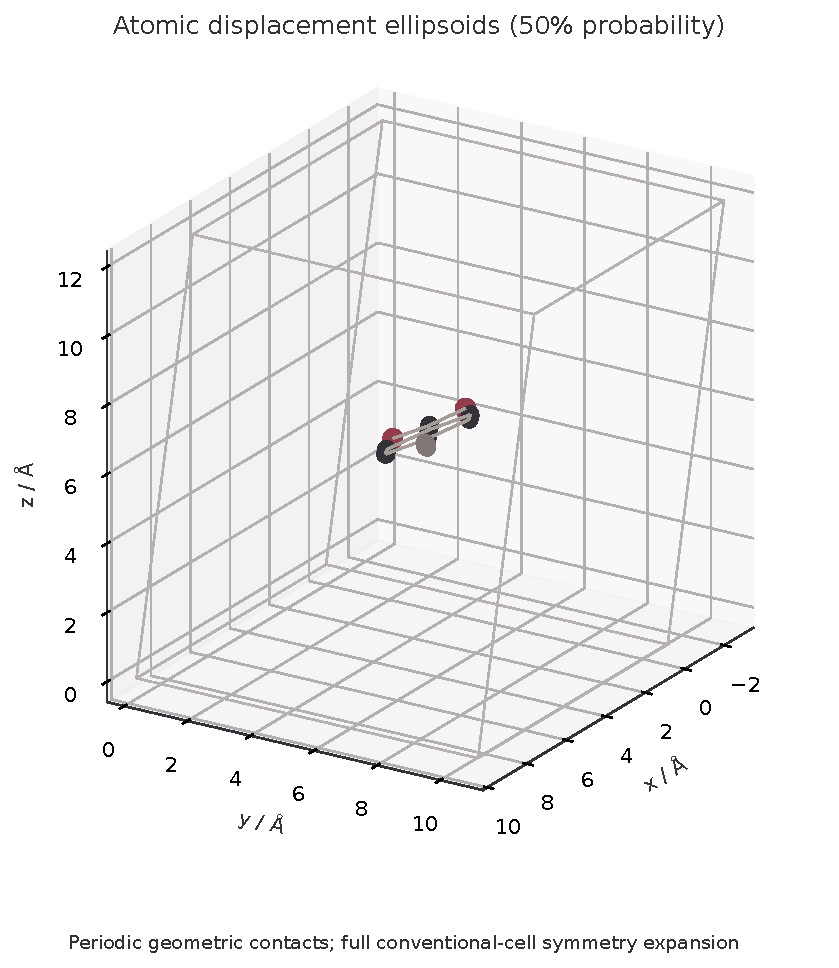
\includegraphics[width=.78\textwidth]{figures/structure_ellipsoids.pdf}
\caption{含各向异性 Br 位点的合成示例之 50\% 位移椭球。晶胞按真实非正交矩阵绘制；图中连接按元素半径与距离生成几何接触候选，不代表独立的化学键价判定。该图对应附录中的有噪声示例，并非实验结构。}
\end{figure}

\section{CIF 张量到笛卡尔张量}
CIF 与 SHELX 常将位移指数写作~\cite{cif_u}
\begin{equation}
T_h=\exp\left[-2\pi^2h^{\mathsf T}\mat D\mat U_{\mathrm{CIF}}\mat D h\right],
\qquad \mat D=\diag(|a^*|,|b^*|,|c^*|).
\end{equation}
因为 $\vct g=\mat A^{-\mathsf T}h$，与式~\eqref{eq:dw} 比较可得
\begin{equation}
\mat U_{\mathrm{cart}}=\mat A\mat D\mat U_{\mathrm{CIF}}\mat D\mat A^{\mathsf T}.
\label{eq:ucif}
\end{equation}
在斜晶胞中，直接把文件中的 $U_{ij}$ 当作笛卡尔协方差来画椭球，会同时改变方向和大小。实现通过不同反射的二次型保持不变来验证式~\eqref{eq:ucif}。

\section{常规差值电子密度}
给定精修模型和强度尺度 $k$，定义显示用幅度
\begin{equation}
F_{o,h}=\sqrt{\max(y_h/k,0)},\qquad
u_h=\begin{cases}F_{c,h}/|F_{c,h}|,&|F_{c,h}|>0,\\1,&|F_{c,h}|=0.\end{cases}
\end{equation}
常规无权重差值图与 $2F_o-F_c$ 图的系数为
\begin{equation}
C_h^{\Delta}=(F_{o,h}-|F_{c,h}|)u_h,
\qquad
C_h^{2o-c}=(2F_{o,h}-|F_{c,h}|)u_h.
\end{equation}
这些图使用模型相位，因此会带有相位偏倚。它们不是模型独立的密度测量，也不是含 $m$、$D$ 或 $\sigma_A$ 权重的统计最优地图。零级系数未知时取零会使显示图的平均密度为零；这一选择影响基线，不改变非零频率提供的结构信息。

精修使用的异常散射复系数一般不严格满足实密度的 Hermitian 条件。为生成实标量图，显示模块平均 $C_h$ 与 $C_{-h}^*$。这一处理仅用于地图，不合并或更改精修中的 Friedel 强度。完全重叠孪晶的观测强度也不属于单一振幅，因而 agent 路线默认不由其平方根直接生成差值密度；需要先有经过验证的去孪晶方案。

\section{从网格到等值面}
三维网格存储分数坐标采样。等值面算法在网格坐标中寻找与给定密度阈值的交点，再将网格位置 $\vct n$ 转为
\begin{equation}
\vct x=\diag(N_1^{-1},N_2^{-1},N_3^{-1})\vct n,
\qquad \vct r=\mat A\vct x.
\end{equation}
对斜晶胞，$\mat A$ 包含剪切和轴间夹角，不能用三个独立的轴长度相乘代替。实现为周期面追加首层切片，再作 marching cubes；追加切片之后，分母仍使用原始 $N_i$，否则整个晶胞会被人为收缩。

\begin{figure}[htbp]
\centering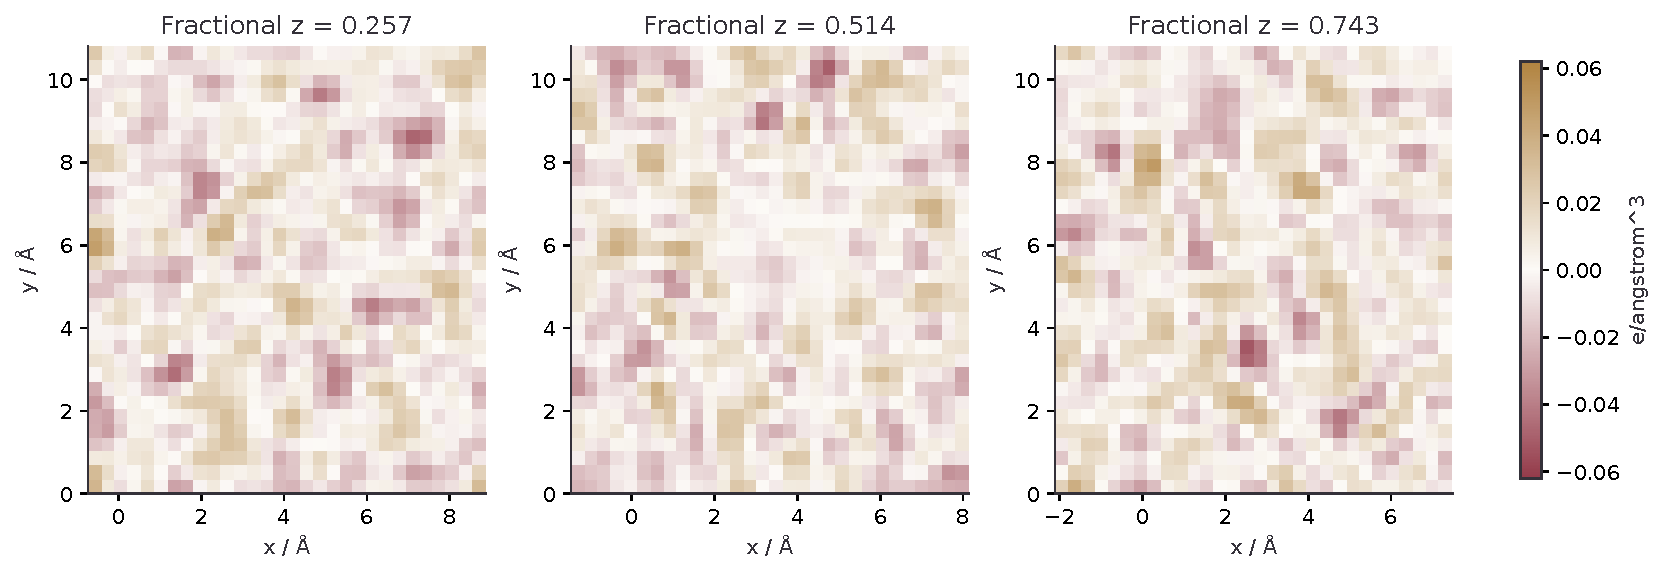
\includegraphics[width=\textwidth]{figures/density_sections.pdf}
\caption{合成示例的差值密度切片。色条给出实际密度单位；默认地图仅使用工作反射。切片和等值面不修改原始观测，缺失系数在显示地图中为零。}
\end{figure}

\section{倒易空间与统计诊断}
倒易空间点应画在 $\vct g_h=\mat B h$，而不是直接把 $h,k,l$ 当作欧氏坐标。颜色可编码标准化残差
\begin{equation}
z_h=\frac{y_h-\mu_h}{\sigma_h}.
\end{equation}
它能显示异常是否集中在特定倒易方向、分辨率范围或反射组。异常点只是需检查的候选，绘图不会自动删除它们。

\begin{figure}[htbp]
\centering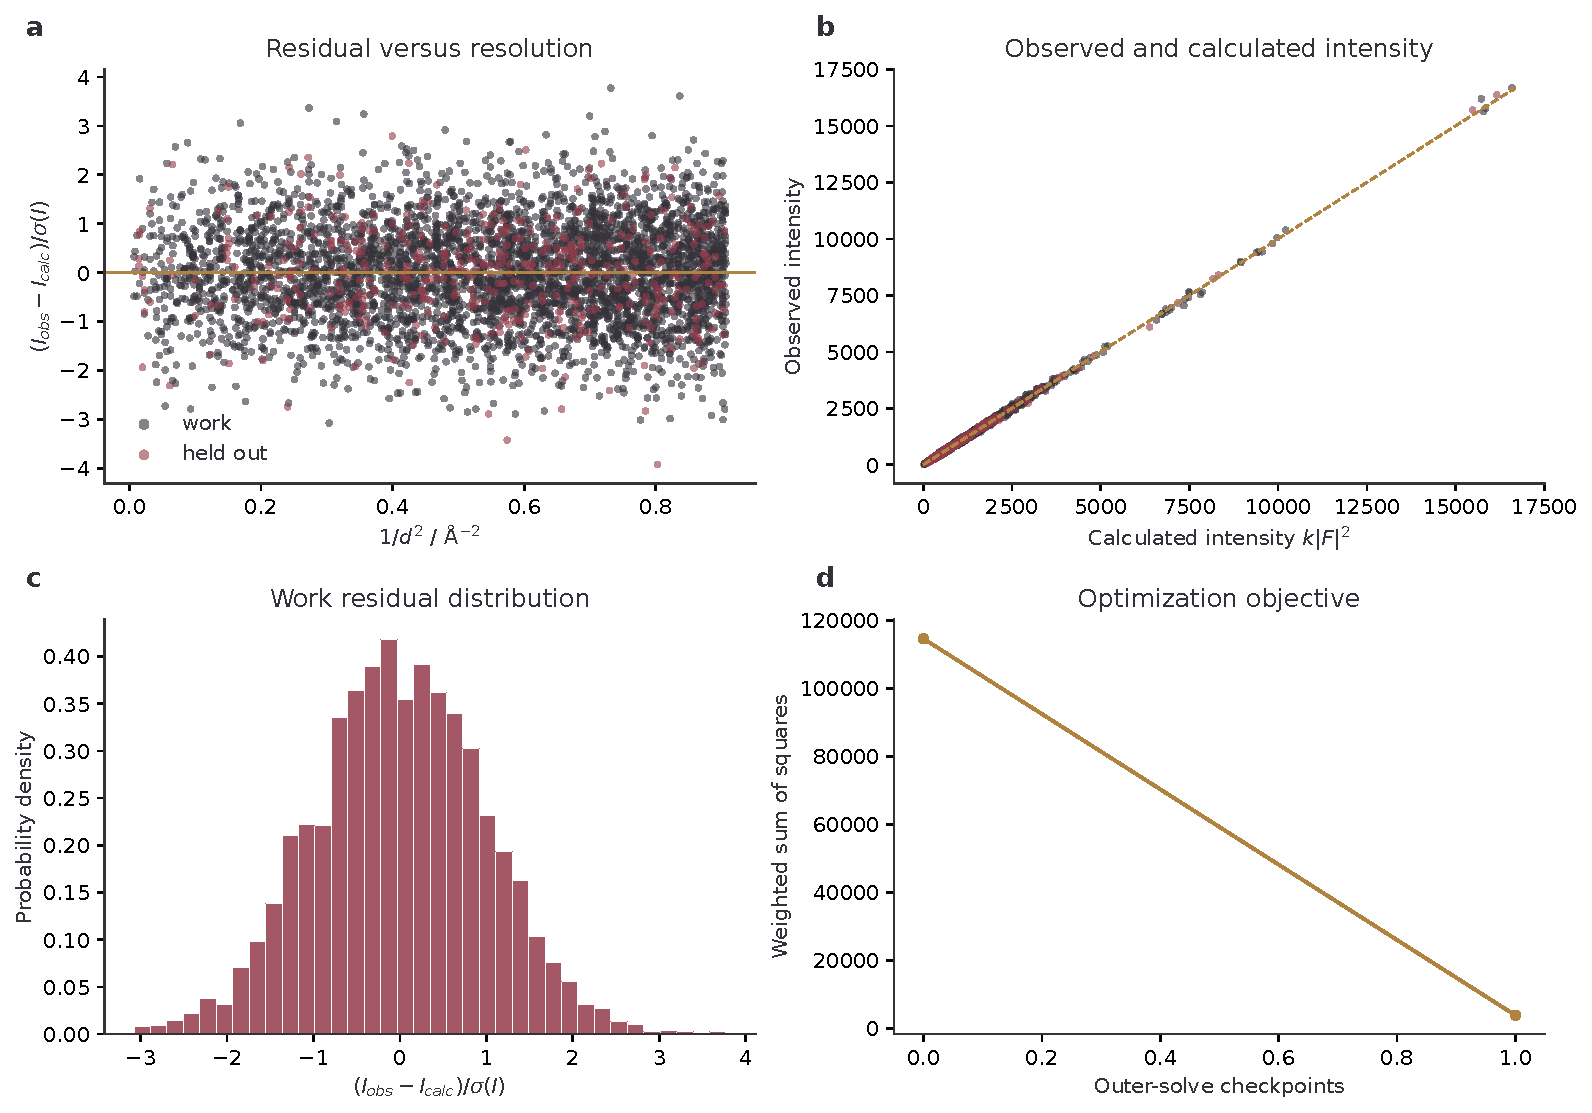
\includegraphics[width=\textwidth]{figures/refinement_diagnostics.pdf}
\caption{有噪声合成示例的强度一致性、分辨率依赖、残差分布及求解检查点。检查点记录初始状态和外层权重求解结束状态，并非每一次内部信赖域迭代。}
\end{figure}

参数相关图采用
\begin{equation}
R_{ij}=\frac{C_{ij}}{\sqrt{C_{ii}C_{jj}}}.
\end{equation}
它反映当前独立参数化下的局部相关。对 Cholesky 或 logit 变量，应结合参数名解释，不能将其直接称为原子笛卡尔坐标之间的相关图。秩亏时不绘制一个由伪逆伪装成的完整参数相关矩阵。

\section{交互图与可发表输出}
交互 HTML 在一个文件中嵌入绘图库，可离线旋转结构、查看原子属性、检查 Miller 指数与密度表面。静态输出采用 SVG 和 PDF 矢量格式，用于报告和论文排版。两者由相同的坐标、张量和数值结果生成，避免交互界面与最终图稿使用不同的科学数据。

绘图的可读性以明确信息为目标：椭球标明概率，地图标明类型和单位，反射图保留指数，合成数据标明来源。更多颜色和表面并不会增加证据；一张图应明确回答一个结构或模型诊断问题。

\chapter{实现契约、执行组织与复杂度}
\section{从数学对象到文件接口}
还原阶段以 EXPT 表示仪器与晶体，以反射表保存观测位置、强度、标记和实验映射；共享像素分析以 JSON/JSONL 保留 contributor、协方差与来源。结构阶段的 \code{Cell}、\code{Atom}、\code{Structure}、\code{Reflections} 分别表示度量、物理原子参数、对称模型和带误差的观测。物理占有率与 SHELX 特殊位置的文件编码在边界转换，不应混成一个数值定义。

所有处理阶段应携带同一个 reader 与单位契约。当前 agent 与旧 MCP 的 DIALS 调用共同使用 \code{dials_command} 和 \code{spotfinding_options}；默认选择 ariadne/matched。读取原始像素的轮廓与 overlap 分析也经过相同 runtime。非 Python dispatcher 在加载科学模块之前给出明确部署错误，避免以错误解释器执行脚本。
\section{核心文件与数学职责}
\begin{longtable}{p{57mm}p{80mm}}
\toprule 源码相对路径或模块 & 职责\\\midrule\endfirsthead
\toprule 源码相对路径或模块 & 职责\\\midrule\endhead
\code{python/src/ariadne/spots.py} & NumPy 检测参考、参数契约与 native dispatch\\
\code{python/src/ariadne/_native.cpp} & float64 检测、缓存、原生积分与并行工作预算\\
\code{threshold_adapter.py} & corrected 像素到 ADU 的临时逆变换\\
\code{lattice_math.py}, \code{ranking.py} & 周期密度、整数基约化、最近点与条件留出评分\\
\code{skills/ariadne-reduction/scripts/} & 以下列出的独立科学脚本所在目录\\
\code{dials_runtime.py} & signed underflow、overflow 和 baseline 解码\\
\code{local_profiles.py} & 局部经验轮廓与 pooled 收缩\\
\code{overlap_integrator.py} & 背景剖面化、有符号 WLS、SVD 与可估计对比\\
\code{constrained_pixels.py} & NNLS、Poisson/PG、QR 与条件剖面区间\\
\code{python/src/ariadne/feedback.py} & 唯一潜变量、低秩 Gaussian 条件化与分组\\
\code{ariadne_xtal/src/ariadne_xtal/} & 结构计算模块所在目录\\
\code{scattering.py}, \code{symmetry.py} & 散射求和、唯一轨道、消光与显式对称操作\\
\code{phasing.py}, \code{refinement.py} & 已知组成求相位、约束参数化与冻结权重精修\\
\code{restraints.py}, \code{feedback.py} & 化学限制与有信息上限的局部 Gaussian 反馈\\
\code{maps.py}, \code{visualization.py} & 物理标度地图、椭球与诊断图\\
\code{compat.py}, \code{shelx.py} & 官方后端调用与严格格式转换边界\\
\bottomrule
\end{longtable}
\section{计算工作与科学接受分别记录}
一个结构状态包括观测、对称假设、原子集合、连续参数、约束、限制和分组。空间群、元素种类、无序数目或孪晶律改变时，应建立新的假设分支。工具调用返回数值和文件，不能由自然语言直接填写“科学成功”。
\begin{table}[htbp]\centering\small
\begin{tabularx}{\textwidth}{p{27mm}X}
\toprule 状态 & 所需证据\\\midrule
执行完成 & 请求成功读取，进程或函数完成并保存预期产物\\
数值收敛 & 目标、步长、梯度或 KKT 满足给定停止条件\\
可辨识 & 去除规范自由度后，数据支持所报告参数或强度对比\\
科学接受 & 化学、对称性、残差、独立检验和替代模型共同支持\\
\bottomrule
\end{tabularx}
\caption{四类判断不能用一个退出码替代。不同模块的初始科学状态字段可能不同，应按实际结果读取。}
\end{table}
原始输入保留，输出写入独立运行目录；输入清单、字节数、程序版本、参数、日志和产物映射用于追溯。本次文档任务不执行任何 SHA-256 计算或验证，也不调用可能隐式执行该操作的旧验证脚本。旧运行记录中的既有字段不作为本报告验收条件。

确定性计划器可以按依赖运行任务，不要求 LLM。可选宿主智能体的职责是选择有类型动作与保留假设证据，实际衍射、优化和误差由数值部件计算。本报告没有用远程模型调用替代任何科学计算。
\section{原生结构算法与官方指令的边界}
原生求相位为已知单胞组成的 $P1$ 多起点电荷翻转或稀疏原子投影。它不包含完整 SHELXT 空间群、原点及元素联立搜索。原生精修支持明确 JSON 模型中的坐标、尺度、ADP、指定占有率和部分约束；一般 HKLF5、全部 AFIX/HFIX、消光、溶剂掩膜和其他完整指令行为由显式官方后端处理。

特别要区分 JSON 功能与 INS 语法：JSON 可表达某个权重或孪晶模型，不意味着 INS 中 WGHT 或 TWIN 已能无损翻译。结构转换白名单之外的科学指令会明确拒绝；原始文件可保留交由官方程序。官方执行成功表示该外部程序完成，不能据此宣称原生功能等价。
\section{主要计算复杂度}
对 $N$ 像素、固定核宽和固定轮数，背景、滑窗及分数主要为 $O(N)$，候选排序和 watershed 的排序阶段约为 $O(M\log M)$，其中 $M$ 为候选像素数。常数成本包括两轮标定、多个背景遍历、相关估计和内存读写。多线程在内存带宽、同步、负载和候选分布约束下不保证线性加速。

对 $m$ 像素、$K$ 个轮廓，稠密 WLS/QR 主要为 $O(mK^2+K^3)$。多次区间求解时增广 QR 将后续固定 Gaussian 目标评估从 $m$ 行降至最多 $K+1$ 行，收益随反复求值次数增加。Gaussian 权重若随参数改变，不能直接重复使用旧压缩因子。

结构因子直接求和约为 $O(HN_a)$，其中 $H$ 为反射数、$N_a$ 为对称展开原子数。通用三点差分 Jacobian 约需 $2P$ 次参数扰动计算，一轮导数约为 $O(PHN_a)$；密集参数系统求解约为 $O(P^3)$。当前通用原生精修使用 SciPy 信赖域与三点差分，理论解析导数没有被表述为已经全量实现。

三维相位恢复网格 $M=N_1N_2N_3$ 的每次 FFT 约为 $O(M\log M)$。独立起点适于并行，同一起点内的迭代具有顺序依赖。低秩反馈全局部分依赖相关秩 $r$，但大的重叠连接组仍需局部稠密处理；因此实现保留矩阵预算而不承诺任意规模。

\chapter{已有验证证据与性能结果}
\section{证据分层与时间范围}
本章汇总仓库已保存的记录，主要为 2026 年 10 月 30--31 日的实验与回归。本次写报告只核对文件、源码与公式，没有再次运行这些科学计算。不同记录的环境、样本和阶段不能合并为一次总实验；旧报告的历史测试数也不与最新针对性回归相加。

合成数据提供已知真值，但正向生成器与被测模型相同的恢复实验，不能独立证明正向模型正确。真实积分参考提供位置与信噪比支持，但不是完整真实性标签。外部程序比较需要模型、权重和时间范围相近；有限指标接近不等于全部指令一致。
\section{合成检测留出集}
验证种子为 200--219，最终测试种子为 300--319；每套各含 20 张 $512\times512$ 图像。规则场景含增益、偏置、读出噪声与掩膜；复杂场景另含环、间隙和尖峰。位置匹配为一对一分配，门限 3 像素，双方均剔除小于 6 像素组件。
\begin{table}[htbp]\centering\small
\begin{tabular}{llrrr}
\toprule 场景 & 方法 & Precision & Recall & F1\\\midrule
规则 & Ariadne matched & 0.9985 & 0.6929 & 0.8181\\
规则 & DIALS Extended，oracle noise & 1.0000 & 0.3633 & 0.5329\\
复杂 & Ariadne matched & 0.9893 & 0.6388 & 0.7763\\
复杂 & DIALS Extended，oracle noise & 0.9969 & 0.4401 & 0.6106\\
\bottomrule
\end{tabular}
\caption{最终测试集，来源为 \code{matched_test.json}。oracle 对照使用真实背景和读出方差构造 $1+r/b$ 方差增益图。}
\end{table}
这些结果支持指定合成条件下召回与 F1 提高，同时精确率略低于强基线。oracle 方差图使对照优于忽略读出噪声的设置，但它不是完整 Poisson--Gaussian 似然。组件下限为 1 的完整结果也保存在 JSON，不能省略该评价条件后推广表中精确率。
\section{真实帧与读取语义}
五个扫描各取 8 帧，共 40 张 $1024\times1536$ 图。参考来自既有双域积分反射，以计算位置、帧范围与 $I/\sigma\ge3$ 定义召回代理。
\begin{table}[htbp]\centering\small
\begin{tabularx}{\textwidth}{Xrrr}
\toprule 方法，同一绝对 underflow 解释 & 召回代理 & 组件数 & 参考支持比例\\\midrule
Ariadne matched & 0.9666 & 2834 & 0.8345\\
DIALS Extended，原 panel gain & 0.6520 & 1314 & 0.9079\\
DIALS Extended，仅有效 gain & 0.8046 & 1799 & 0.8994\\
DIALS Extended，有效 gain 与 offset & 0.8475 & 1978 & 0.8888\\
\bottomrule
\end{tabularx}
\caption{\code{matched_real_absolute.json}，均采用 6 像素下限。参考不完整，最后一列不能称作 precision。}
\end{table}
DIALS 校准对照借用同帧背景估计的 gain/offset，不用参考反射调参；其检测时间不包括 Ariadne 标定成本。位置附近存在旧反射不构成独立真实性证明，缺少旧反射也不等于误检。

在第一扫描第 20 帧，旧 dxtbx 解释使 82,397 个像素多加 64 ADU，占 5.24\%，涉及原值 47--64 ADU。绝对 underflow 解码与 FabIO 语义一致。保留旧解释的另一组检测记录中，Ariadne 召回代理为 0.9714，校准 DIALS 为 0.8618，但 Ariadne 参考支持比例降至 0.7692。读取语义会实质改变候选分布，不能跨解释直接归因于算法质量。
\section{检测速度及逐阶段开销}
最终内核对四张真实帧运行 14 轮，剔除各方法前两次样本；单线程与四工作单元顺序逐轮交换。排除磁盘读取和径向 bins 构造，保留 Python 调用与动态掩膜成本。
\begin{table}[htbp]\centering\small
\begin{tabular}{lr}
\toprule 同轮方法 & 中位时间 / ms\\\midrule
Ariadne matched，单线程 & 163.513\\
Ariadne matched，四工作单元 & 87.195\\
DIALS Extended，复用 C++/flex 输入 & 27.950\\
DIALS Extended，含 NumPy/flex 转换 & 32.631\\
\bottomrule
\end{tabular}
\caption{\code{matched_timing_final.json}。四工作单元相对单线程约快 1.88 倍，仍比 DIALS C++ 慢约 3.12 倍。}
\end{table}
四工作单元阶段中位数依次为 load 4.25、background 18.38、calibration 24.28、noise 16.18、scores 13.37、basins 4.45 ms。阶段中位数之和不必等于总时间中位数，背景和校准仍为主要热点。Ariadne 执行额外背景、标定、相关修正和区域分割，这说明工作量不同，但不改变速度目标未达到的事实。

记录时机器存在持续外部 CPU 负载，因此不可用早期更空闲记录的绝对时间计算本轮收益。现有优化没有证明进一步保持精度的加速已不可能；这里只陈述当前测得性能。
\section{Gaussian 增广 QR 的完整求解收益}
基准使用固定种子 6817、三个重叠 Gaussian 轮廓、异方差固定噪声、背景像素与掩膜。每组五次交替计时覆盖完整拟合、所有分量及总量剖面区间；对照仅将压缩函数换为原像素路径。
\begin{table}[htbp]\centering\small
\begin{tabular}{rrrr}
\toprule 请求信号行数 & 原像素 / ms & QR / ms & 加速比\\\midrule
64 & 12.630 & 12.743 & 0.99\\
700 & 19.191 & 15.979 & 1.20\\
1600 & 20.063 & 14.227 & 1.41\\
12000 & 50.894 & 14.041 & 3.62\\
60000 & 212.244 & 18.597 & 11.41\\
\bottomrule
\end{tabular}
\caption{\code{gaussian_profile_compression.json}，固定方差 Gaussian NNLS 合成数据，单进程及单线程。}
\end{table}
25 对结果的最大区间端点差为 $1.09\times10^{-11}$、强度差 $3.46\times10^{-11}$、目标差 $1.46\times10^{-11}$，原像素空间投影梯度不超过 $7.203\times10^{-13}$。这些是有限案例中的浮点证据，与式~\eqref{eq:augmentedqr} 的代数恒等式共同支持该优化；它们不表示 Poisson/PG 或整条真实流程加速相同倍数。
\section{32 帧真实链路与结构入口}
真实 Store、Context 与生产 backend 已执行以下有限路线。
\begin{table}[htbp]\centering\small
\begin{tabularx}{\textwidth}{l r X}
\toprule 阶段 & 时间 / s & 输出\\\midrule
import & 4.586 & 同一原始 ADU 读取契约的 EXPT\\
matched find\_spots & 8.875 & 389 个斑点\\
index & 10.476 & 254/389 归属一个晶格\\
refine & 8.088 & 原生 DIALS 几何精修输出\\
integrate & 8.431 & 1048 行，保留 144 个负 sum 强度\\
\bottomrule
\end{tabularx}
\caption{\code{reduction_path_run2/reduction_path.json}。时间含进程、I/O 与计算，无同范围整链 DIALS 基线。}
\end{table}
首帧 raw 与 FabIO 逐像素相等，corrected 逆变换后检测 mask 与 raw 一致。该单位检查显式使用 offset/readout，且关闭检测自校准，因此不是探测器实验标定。原数据为双域，此有限单晶路径验证软件衔接；它尚未覆盖完整多扫描约化、缩放和多域吸收/重叠验收。

另取既有完整积分的原 crystal 0，共 8823 行、1188 个负 sum 强度，使用现有 CIF 的组成 C20 H16 Co N2 O5 导出，保留 1092 个负 HKL 行。真实 SHELXT 生成三组 RES/HKL，候选 R1 为 0.270、0.240、0.249；组成和空间群尚需判断。这条证据来自旧积分，不能接到上述 32 帧后宣称新 raw 到完整结构已经成功。
\section{结构精修与真实 SHELXL 对照}
\code{xtal_shelxl.json} 保存三种受控模型的真实进程比较。均使用固定晶胞、固定占有率、各向同性 ADP 和显式异常散射。没有自由反射集，限制残差数为零。
\begin{table}[htbp]\centering\small
\begin{tabularx}{\textwidth}{Xrrrr}
\toprule 案例 & 反射数 & 原生 $wR_2$ & SHELXL $wR_2$ & 最大坐标差 / $\angstrom$\\\midrule
FeN$_4$ 公开实测 & 71 & 0.081480 & 0.0815 & 0.001957\\
$P\bar1$ 三原子合成 & 665 & 0.024887 & 0.0248 & 0.0000827\\
$P\bar1$ 八原子合成 & 665 & 0.020725 & 0.0207 & 0.0000772\\
\bottomrule
\end{tabularx}
\caption{有限相同模型中的数值接近；不包含各向异性、无序、占有率或孪晶分数的完整官方等价性验证。}
\end{table}
FeN$_4$ 观测来自 Bykov 等的公开数据\cite{fen4_2018}，原生强反射 $R_1=0.04031575$、SHELXL 为 0.0404。当前记录的原生热内核中位时间为 84.90 ms，新 Python 进程为 337.36 ms，SHELXL 新进程为 78.42 ms。该主机为 arm64，SHELXL 为 x86\_64/Rosetta。三个案例的热内核/SHELXL 进程时间比分别约 1.08、1.41、7.16，新 Python 进程比约 4.30、4.36、9.91；范围不同，应分别报告，不支持原生更快的结论。

同一记录还有无噪声四碳 $P1$、4540 条反射的求相位案例：原生峰恢复 RMS 为 0.0107474 $\angstrom$，精修后为 $1.42\times10^{-8}$ $\angstrom$。SHELXT 最佳结果约为 $4.63\times10^{-16}$ $\angstrom$，两者搜索空间不等价。该实例的极小误差源于无噪声和匹配正向模型，不是实验坐标精度或一般成功率。
\section{针对性回归与证据边界}
最终检测与接口回归日志记录 90 项通过、45 个子测试通过、2 项 MCP 测试在主环境跳过；后两项在带既有 MCP 运行库的环境单独通过。三条既有 SWIG 类型弃用警告保留。六组合成与四张真实帧在单线程/四工作单元共 20 组对照中布尔像素差为零；噪声统计最大绝对差约 $2.28\times10^{-11}$。

这些结果验证实际用例的一致性，不证明任意阈值附近输入的浮点位级恒等。DIALS 3.30.1 补丁已保存精确行号应用检查和语法检查证据；零上下文 hunk 使用 \code{git apply --unidiff-zero}。历史汇总 \code{summary.json} 属于另一批运行，不把其 369/143 等数量叠加到本章针对性回归。

当前证据支持数学部件、有限案例数值一致性、部分检测质量提升和具体 Gaussian 加速；尚未建立全数据多域结构的最终科学接受，也没有多化学体系解析成功率、跨平台性能排名或全面优于 DIALS/SHELX 的结论。

\appendix
\chapter{源码映射与复现说明}
\section{编译本报告}
本报告为 UTF-8 中文 LaTeX 工程，使用 TeX Live 的 \code{ctexbook} 与 Fandol 字体，不依赖下载字体。\code{chapters/} 保存正文，\code{figures/} 保存从参考报告沿用的三幅已有矢量图，\code{references.tex} 为可读参考文献。所有章节和配图保持相对路径，可离线编译。
\begin{lstlisting}
xelatex -no-shell-escape -interaction=nonstopmode -halt-on-error Ariadne_Mathematical_Technical_Report.tex
\end{lstlisting}
同一命令运行两次以完成目录、文献与交叉引用。首次生成的辅助文件不属于最终科学数据；交付压缩包包含源文件、已有图版、说明与 PDF，不包含实测反射表、原始帧、数据库和本地结构候选。
\section{检测与积分证据文件}
下列路径相对于仓库根目录 \code{reports/current_validation/}。
\begin{longtable}{p{65mm}p{72mm}}
\toprule 文件 & 可核对内容\\\midrule\endfirsthead
\toprule 文件 & 可核对内容\\\midrule\endhead
\code{matched_validation.json} & 验证种子、参数与全部方法输出\\
\code{matched_test.json} & 最终合成种子、组件下限与一对一匹配统计\\
\code{matched_real_absolute.json} & 绝对 underflow 语义下真实帧检测\\
\code{matched_real_dxtbx.json} & 原 dxtbx 解释下独立对照\\
\code{matched_timing_final.json} & 每轮时间、单线程/四工作单元与阶段时间\\
\code{matched_parity.json} & 各例 mask 差与噪声模型浮点差\\
\code{gaussian_profile_compression.json} & QR 完整拟合、区间、KKT 与原始计时\\
\code{reduction_path_run2/reduction_path.json} & 32 帧实际命令、输出、旧积分导出和限制\\
\code{xtal_shelxl.json} & 真实 SHELXL 对照、模型与平台限制\\
\code{matched_regression_output.txt} & 实际针对性回归输出\\
\bottomrule
\end{longtable}
\section{针对性复现入口}
以下命令用于解释已有记录的入口，\textbf{本次文档编写没有执行它们}。需要匹配 DIALS 科学环境、源码路径与原始输入；含真实数据的运行应写入新的本地目录。
\begin{lstlisting}
python benchmarks/matched_spots.py --split test --output /path/to/new_matched_test.json
python benchmarks/matched_spots_timing.py --experiments /path/to/integrated.expt --compare-threads --repeat 20 --output /path/to/new_timing.json
python benchmarks/gaussian_profile_compression.py
\end{lstlisting}
\code{matched_spots_parity.py} 对照 NumPy/native 分数模型与选择输出。\code{validate_reduction_path.py} 使用真实生产 backend 验证限定帧路线，需要明确 source EXPT、source refl、composition CIF 和新输出目录。它不能仅凭存在输入文件就替代全扫描科学验收。应在明确需要复验时运行对应检查，避免与任务无关的重复构建或测试。
\section{实现中需要准确解释的细节}
原生 occupancy-sum 约束目前只接受 $0<t\le1$，要求成员均可精修、初始占有率严格正并满足总和，且不与其他占有率约束重叠；一般线性约束的理论不代表任意目标和均已实现。角度限制的数值单位为度。ADP 相似残差的非对角分量乘 $\sqrt2$，使平方和对应 Frobenius 范数。距离相似组以第一对为参照。

各向异性位移采用正定参数化或特殊位置不变子空间，但 \code{u_min/u_max} 不等于最终每个特征值都具有相同上下界。活动边界在内部用于警告与相关 s.u. 置空，当前结果并不逐变量序列化完整 \code{active_mask}。

agent 遇完全重叠孪晶模型时跳过常规差值图；直接底层 \code{difference_map()} API 没有孪晶参数来自动检查这一条件。因此调用者必须确保输入属于可解释的单一幅度模型。地图显示采用的截断开方不会改变精修中保留的负强度。

波长不自动为每个元素加载异常散射修正。原生模型的 $f',f''$ 默认为零；使用显式色散或指定适配器时应记录来源。特殊位置只累加不同位置，并按稳定子平均变换的位移张量；对一般位置的全部操作求和不能直接复制到特殊位置。

\begin{thebibliography}{99}
\addcontentsline{toc}{chapter}{参考文献}
\latinfont
\bibitem{shelxt2015} Sheldrick, G. M. SHELXT---Integrated space-group and crystal-structure determination. \textit{Acta Crystallographica A} \textbf{71}, 3--8 (2015). \href{https://doi.org/10.1107/S2053273314026370}{doi:10.1107/S2053273314026370}.
\bibitem{shelxl2015} Sheldrick, G. M. Crystal structure refinement with SHELXL. \textit{Acta Crystallographica C} \textbf{71}, 3--8 (2015). \href{https://doi.org/10.1107/S2053229614024218}{doi:10.1107/S2053229614024218}.
\bibitem{shelxl_instructions} SHELX. Alphabetical list of SHELXL instructions. \url{https://shelx.uni-goettingen.de/shelxl_html.php}. 参考报告所列来源；本次未重新访问网页。
\bibitem{chargeflip2004} Oszl\'anyi, G. and S\"ut\H{o}, A. Ab initio structure solution by charge flipping. \textit{Acta Crystallographica A} \textbf{60}, 134--141 (2004). \href{https://doi.org/10.1107/S0108767303027569}{doi:10.1107/S0108767303027569}.
\bibitem{sayre1952} Sayre, D. The squaring method: a new method for phase determination. \textit{Acta Crystallographica} \textbf{5}, 60--65 (1952). \href{https://doi.org/10.1107/S0365110X52000137}{doi:10.1107/S0365110X52000137}.
\bibitem{direct_methods} IUCr. An introduction to direct methods. IUCr Teaching Pamphlets. \url{https://www.iucr.org/what-we-do/education/pamphlets/introduction-direct-methods}. 参考报告所列来源；本次未重新访问网页。
\bibitem{rigu2012} Thorn, A., Dittrich, B. and Sheldrick, G. M. Enhanced rigid-bond restraints. \textit{Acta Crystallographica A} \textbf{68}, 448--451 (2012). \href{https://doi.org/10.1107/S0108767312014535}{doi:10.1107/S0108767312014535}.
\bibitem{parsons2013} Parsons, S., Flack, H. D. and Wagner, T. Use of intensity quotients and differences in absolute structure refinement. \textit{Acta Crystallographica B} \textbf{69}, 249--259 (2013). \href{https://doi.org/10.1107/S2052519213010014}{doi:10.1107/S2052519213010014}.
\bibitem{fen4_2018} Bykov, M., Khandarkhaeva, S., Fedotenko, T., Sedmak, P., Dubrovinskaia, N. and Dubrovinsky, L. Synthesis of FeN$_4$ at 180 GPa and its crystal structure from a submicron-sized grain. \textit{Acta Crystallographica E} \textbf{74}, 1392--1395 (2018). \href{https://doi.org/10.1107/S2056989018012161}{doi:10.1107/S2056989018012161}. Original supporting data and attribution are retained in the source package.
\bibitem{gemmi_scattering} Gemmi developers. Scattering: form factors, anomalous scattering and direct summation. \url{https://gemmi.readthedocs.io/en/latest/scattering.html}. 既有报告引用；软件版本按各验证记录分别读取。
\bibitem{gemmi_symmetry} Gemmi developers. Crystallographic symmetry and space-group operations. \url{https://gemmi.readthedocs.io/en/latest/symmetry.html}. 参考报告所列来源；本次未重新访问网页。
\bibitem{gemmi_grid} Gemmi developers. Grids and maps. \url{https://gemmi.readthedocs.io/en/latest/grid.html}. 参考报告所列来源；本次未重新访问网页。
\bibitem{cif_u} IUCr COMCIFS. Core CIF dictionary: \code{_atom_site_aniso_U_} definitions. \url{https://www.iucr.org/__data/iucr/cifdic_html/1/cif_core.dic/Iatom_site_aniso_U_.html}. 参考报告所列来源；本次未重新访问网页。
\bibitem{scipy_lsq} SciPy developers. \code{scipy.optimize.least_squares}: nonlinear least squares with bounds. \url{https://docs.scipy.org/doc/scipy/reference/generated/scipy.optimize.least_squares.html}. 既有报告引用；软件版本按各验证记录分别读取。
\bibitem{mcp_sdk} Model Context Protocol. Official Python SDK and server documentation. \url{https://github.com/modelcontextprotocol/python-sdk}; \url{https://py.sdk.modelcontextprotocol.io/}. 既有报告引用；本次未运行协议测试。
\bibitem{shelx_distribution} SHELX distribution and registration information, linked by CCP4. \url{https://www.ccp4.ac.uk/download/shelx.php}; \url{https://shelx.uni-goettingen.de/}. 参考报告所列来源；本次未重新访问网页。

\bibitem{dials} Winter, G., Waterman, D. G., Parkhurst, J. M., et al. DIALS: implementation and evaluation of a new integration package. \textit{Acta Crystallographica D} \textbf{74}, 85--97 (2018). \href{https://doi.org/10.1107/S2059798317017235}{doi:10.1107/S2059798317017235}.
\bibitem{geometry} Waterman, D. G., Winter, G., Gildea, R. J., et al. Diffraction-geometry refinement in the DIALS framework. \textit{Acta Crystallographica D} \textbf{72}, 558--575 (2016). \href{https://doi.org/10.1107/S2059798316002187}{doi:10.1107/S2059798316002187}.
\bibitem{fabio} FabIO developers. Bruker100 image reader, \code{bruker100image.py}. \url{https://github.com/silx-kit/fabio/blob/main/src/fabio/bruker100image.py}. 解码语义参照既有核查记录，本次未重新访问网页。
\bibitem{local_evidence} Ariadne project. \textit{Self-calibrated matched detection, fused numerical kernels and Gaussian profile compression: stored validation records}. \code{reports/current_validation/}, source baselines \code{cec63ba186a1843389b1ae161944388304ff1cdd} and \code{25d228b2f587cf2ba464bd64c89ee1739855fe68}, 2026-10-31 to 2026-11-02. 本地计算记录，不是同行评审论文。
\bibitem{reference_pdf} \textit{单晶结构求解与精修的数学基础：面向智能体的 Ariadne-Xtal 计算体系}. 用户提供的 47 页 PDF，2026-10-30；对应原 LaTeX 工程位于 \code{ariadne_xtal/docs/}。本报告复用其理论章节与三个已有合成图版，并补写数据还原、反馈、实现与验证章节。

\end{thebibliography}

\end{document}
